    \documentclass[conference,9pt]{IEEEtran}
\IEEEoverridecommandlockouts
% The preceding line is only needed to identify funding in the first footnote. If that is unneeded, please comment it out.
%Template version as of 6/27/2024

\usepackage{cite}
\usepackage{amsmath,amssymb,amsfonts}
\usepackage{algorithmic}
\usepackage{graphicx}
\usepackage{textcomp}
\usepackage{xcolor}
\usepackage{verbatim}
\usepackage{framed}
\usepackage{listings}
\usepackage{multirow}
\usepackage{booktabs}
\usepackage{float}
% \usepackage{appendix}
\def\BibTeX{{\rm B\kern-.05em{\sc i\kern-.025em b}\kern-.08em
    T\kern-.1667em\lower.7ex\hbox{E}\kern-.125emX}}

\newcommand{\tabincell}[2]{\begin{tabular}{@{}#1@{}}#2\end{tabular}}

% reduce space above and below floats (tables & figures)
\setlength{\floatsep}{3pt}     % between floats
% \setlength{\textfloatsep}{12pt plus 3pt minus 3pt} % between floats and text (top/bottom)
% \setlength{\intextsep}{8pt plus 1pt minus 1pt}    % between in-text floats and text
\setlength{\intextsep}{3pt} % Adjust space above and below in-text floats
\setlength{\textfloatsep}{3pt} % Adjust space between floats and text

\begin{document}

\title{
% NL2SVA: LLM-based SystemVerilog Assertion Generation from Natural Language
Hybrid-NL2SVA: Integrating RAG and Finetuning for LLM-based NL2SVA
}

\author{%
{\normalsize Weihua Xiao, Derek Ekberg, Siddharth Garg, Ramesh Karri}\\
{\normalsize NYU Tandon School of Engineering, Brooklyn, NY, USA}\\
{\normalsize Emails: \{wx2356, dhe9940\}@nyu.edu, siddharth.j.garg@gmail.com, rkarri@nyu.edu}
}

% \author{\IEEEauthorblockN{1\textsuperscript{st} Given Name Surname}
% \IEEEauthorblockA{\textit{dept. name of organization (of Aff.)} \\
% \textit{name of organization (of Aff.)}\\
% City, Country \\
% email address or ORCID}
% \and
% \IEEEauthorblockN{2\textsuperscript{nd} Given Name Surname}
% \IEEEauthorblockA{\textit{dept. name of organization (of Aff.)} \\
% \textit{name of organization (of Aff.)}\\
% City, Country \\
% email address or ORCID}
% \and
% \IEEEauthorblockN{3\textsuperscript{rd} Given Name Surname}
% \IEEEauthorblockA{\textit{dept. name of organization (of Aff.)} \\
% \textit{name of organization (of Aff.)}\\
% City, Country \\
% email address or ORCID}
% \and
% \IEEEauthorblockN{4\textsuperscript{th} Given Name Surname}
% \IEEEauthorblockA{\textit{dept. name of organization (of Aff.)} \\
% \textit{name of organization (of Aff.)}\\
% City, Country \\
% email address or ORCID}
% \and
% \IEEEauthorblockN{5\textsuperscript{th} Given Name Surname}
% \IEEEauthorblockA{\textit{dept. name of organization (of Aff.)} \\
% \textit{name of organization (of Aff.)}\\
% City, Country \\
% email address or ORCID}
% \and
% \IEEEauthorblockN{6\textsuperscript{th} Given Name Surname}
% \IEEEauthorblockA{\textit{dept. name of organization (of Aff.)} \\
% \textit{name of organization (of Aff.)}\\
% City, Country \\
% email address or ORCID}
% }
\IEEEoverridecommandlockouts
\IEEEpubid{\makebox[\columnwidth]{979-8-3315-3762-3/25/\$31.00~\copyright2025 IEEE \hfill} \hspace{\columnsep}\makebox[\columnwidth]{ }}

\maketitle
% \IEEEpubidadjcol

\begin{abstract}
\textit{SystemVerilog Assertion}s (\textit{SVA}s) are critical for verifying the correctness of hardware designs, but manually writing them from natural language property descriptions, i.e., \textit{NL2SVA}, remains a labor-intensive and error-prone task. 
Recent advances in \textit{large language model}s (\textit{LLM}s) offer opportunities to automate this translation. 
However, existing models still struggle with understanding domain-specific syntax and semantics. 
To enhance LLM performance in NL2SVA, we propose a customized \textit{retrieval-augmented generation} (\textit{RAG}) framework and a synthetic fine-tuning dataset that together improve LLM's performance. 
% propose a customized \textit{Retrieval-Augmented Generation} (\textit{RAG}) framework that systematically improves both the \textit{database construction} and \textit{retrieval process} of traditional RAG pipelines, and further refines the generated assertions. 
% First, we introduce a \textit{dynamic splitting technique} to construct a context-preserving retrieval database by semantically segmenting SystemVerilog textbooks. 
% Second, we develop \textit{HybridRetrieval}, a retrieval process that combines \textit{global semantic retrieval} with \textit{keyword-guided retrieval} to extract relevant SVA operator-specific contexts. 
% Third, we propose an \textit{SVA operator-based rechecking flow} to validate and correct the SVA operator use in LLM-generated assertions. 
Our RAG framework (i) constructs a context-preserving database via \textit{dynamic splitting technique}, (ii) combines global semantic retrieval with keyword-guided retrieval to extract SVA operator-related contexts via \textit{HybridRetrieval}, and (iii) validate and correct the use of SVA operators in LLM-generated SVAs via \textit{SVA operator-based rechecking}.
To further improve lightweight models over NL2SVA, our fine-tuning dataset provides \textit{prompt-guided explanation}s that teach LLMs the layer-by-layer construction process of concurrent SVAs, enabling supervised fine-tuning that greatly improves syntax and functionality accuracy.
To evaluate the performance of LLMs over NL2SVA, we construct the largest evaluation dataset for NL2SVA, comprising $40$ Verilog designs and $229$ formally verified SVAs with detailed annotations.
% Experimental results show that  RAGSVAG framework can improve the number of generated functionality match SVAs by $58.42\%$ over \textit{GPT-4o mini}. 
Experimental results show that our customized RAG framework increases the number of functionality matched SVAs by $58.42 \%$ over \textit{GPT-4o-mini}, while \textit{Qwen2.5-Coder-7B-Instruct} fine-tuned on our fine-tuning dataset and integrated with HybridRetrieval achieves a $59.05 \%$ over the base Qwen model.
% RAGSVAG code and evaluation dataset are released at https://github.com/FCHXWH823/RAG-aided-Assertion-Generation.
% To rigorously evaluate the effectiveness of our framework, we construct the largest evaluation dataset, to our knowledge, for natural language to SVA translation, consisting of $40$ Verilog designs and $229$ formally verified SVAs with detailed annotations.
% To enhance LLM performance in SVA generation, we propose \textit{RAG-SVAGen}, a \textit{Retrieval-Augmented Framework} that improves both the database construction and retrieval process of the traditional RAG pipeline. 
% First, we introduce a \textit{dynamic splitting technique} to construct a context-preserving retrieval database by semantically segmenting code snippets from SystemVerilog textbooks. 
% Second, we develop \textit{HybridRetrieval}, a retrieval process that combines \textit{global semantic retrieval} with \textit{keyword-guided retrieval} to enhance the retrieval quality. 
% To rigorously evaluate our framework, we construct the largest evaluation dataset to date for natural language to SVA translation, consisting of 40 Verilog designs and 229 formally verified SVAs with detailed annotations. Experimental results demonstrate that RAG-SVAGen significantly improves functionality match rates compared to strong LLM baselines, highlighting the effectiveness of retrieval-augmented techniques tailored for SVA synthesis.
% To improve LLM performance in SVA generation, we propose \textit{RAG-SVAGen}, a \textit{Retrieval-Augmented Framework} that enhances LLMs by retrieving relevant domain-specific context.
% At the core of RAG-SVAGen, we construct a retrieval database from SystemVerilog textbooks by proposing a \textit{dynamic splitting technique}, which can help reducing unnecessary or irrelevant content in the database. 
% To further enhance retrieval quality, we develop \textit{HybridRAG}, which combines \textit{global semantic retrieval} with \textit{keyword-guided retrieval}. 
% Additionally, we propose an \textit{SVA operator-based rechecking flow} to further refine LLM-generated assertions by verifying the correctness of operator usage.
% To rigorously evaluate the effectiveness of our framework, we construct a comprehensive evaluation dataset, which is the largest one for natural language to SVA translation to our knowledge, consisting of $40$ Verilog designs and $229$ formally verified SVAs with detailed annotations. 
% Experimental results show that our proposed RAG framework can improve the number of generated functionality match assertions by $29.1\%$ over the OpenAI CodeX model in the prompt assertion generation task.
\end{abstract}

\IEEEpubidadjcol
\begin{IEEEkeywords}
Large Language Model, SystemVerilog Assertion, Evaluation Dataset, Retrieval-Augmented Generation, Fine-tuning
\end{IEEEkeywords}

\section{Introduction}
\label{sec:introduction}
% Hardware verification is a critical phase in the chip design cycle, often taking up to $70\%$ of the development time~\cite{Farahmandi19}.
\textit{SystemVerilog Assertion}s (\textit{SVA}s) are essential tools in hardware verification, formally specifying expected design behaviors, namely the \textit{design properties}, and serving as embedded checkers that continuously validate the implementation against its specification~\cite{Witharana22,SystemVerilog18}.
% \textit{SystemVerilog Assertion}s (\textit{SVA}s) are essential tools in hardware verification, formally specifying expected design behaviors, i.e., \textit{design properties}, and serving as embedded checkers that continuously validate the implementation against its specification~\cite{Witharana22,SystemVerilog18}.
% For over a decade, \textit{Assertion-Based Verification} (\textit{ABV}) has become the de facto standard for verifying the functional and security properties of hardware designs~\cite{Witharana22}.
% Within this process, \textit{SystemVerilog Assertions} (\textit{SVAs}) have become essential tools for ensuring correctness in complex designs.
% SVAs are used to formally specify the expected behaviors, i.e., the \textit{design propertie}s, and act as embedded checkers that continuously validate the design against its specification.
% These assertions are violated whenever the actual design behaviors deviate from the expected ones specified in the assertions, and errors will be reported during verification~\cite{SystemVerilog18}.
However, writing SVAs manually is difficult, which consists of two sub-tasks~\cite{Vasudevan10,Witharana23}.
The first task is to extract intended properties, described in natural language, from hardware designs and detailed specification documents. 
% However, as designs grow larger and more complex, it becomes increasingly challenging to capture all important properties needed to cover every necessary checking case.
Once these are identified, the second task is to implement these natural language properties as SVAs, i.e., the NL2SVA task. 
% This task is also challenging because it demands deep domain expertise in both the hardware design’s functionality and the syntax of SVAs.
% These challenges often lead to incomplete verification coverage, where key behaviors may be overlooked, and increase the likelihood of human errors in manually generated SVAs, resulting in undetected bugs. 
% This underscores the need for an automated approach to SVA generation~\cite{Yan25}.
Recent advances in \textit{Natural Language Processing} (\textit{NLP}) or \textit{Large Language Models} (\textit{LLMs}), such as \textit{GPT}-$4$\textit{o} and \textit{DeepSeek}, have shown promising potential in automating both sub-tasks~\cite{Radu24,Mali24}.

For the first sub-task of property extraction, several recent works have explored different techniques~\cite{Yan25,parthasarathy2021spectosva,Meng24}.
\textit{AssertLLM}~\cite{Yan25} proposes a multi-LLM framework that processes the complete specification document to extract design properties for each architectural signal.
\textit{SpecToSVA}~\cite{parthasarathy2021spectosva} trains a machine-learning-based sentence classifier to automatically detect property-relevant sentences from specification documents, reducing manual effort in identifying verification properties.
\textit{NSPG}~\cite{Meng24} introduces a fine-tuned domain-specific LLM to  mine hardware security properties from specification documents.
% Recent advances in \textit{Natural Language Processing} (\textit{NLP}) or \textit{Large Language Models} (\textit{LLMs}), such as \textit{GPT}-$4$\textit{o} and \textit{DeepSeek}, have shown promising potential in automating both sub-tasks~\cite{Radu24}. 
% For the first sub-task, approaches mainly utilize LLM pipelines to extract relevant sentences from specification documents~\cite{Yan25}.
% In this paper, we focus specifically on the second sub-task.

% Several recent works have explored automating both sub-tasks. Techniques such as natural language processing models and specification mining tools have been proposed to assist in property extraction [7], [8]. Separately, approaches using large language models (LLMs) have been introduced to generate SVAs from extracted property descriptions [9], [10].

Recent works have also explored automating the NL2SVA sub-task using both \textit{rule-based} and \textit{LLM-based} methods. Traditional rule-based methods, such as \textit{GLaST}~\cite{Harris16} and \textit{Ease}~\cite{Krishnamurthy19}, rely on manually crafted grammars, rules, or templates, but struggle to generalize across diverse specifications and require substantial manual effort. 
More recently, LLM-based approaches like \textit{nl2spec}~\cite{Cosler23} introduce interactive prompting frameworks where engineers refine LLM-suggested subformulas to improve accuracy, but it depends heavily on human intervention and careful prompt design. 
AssertLLM also proposes a multi-LLM pipeline and incorporates a \textit{retrieval-augmented generation} (\textit{RAG}) component to assist NL2SVA; 
however, it just uses the generic retrieval method, and focuses only on syntax correctness and \textit{Formal Property Verification} (\textit{FPV}) pass of generated SVAs, without evaluating functionality match of generated SVAs to the natural language property description.
In~\cite{wu2025}, the authors first convert the natural language description into an intermediate formal representation, and then decompose that representation into fragments, translates each fragment into its corresponding SVA, and finally combines them into a complete assertion.
\cite{Shahidzadeh24} uses pairs of SVAs and natural language explanations to finetune \textit{GPT-3.5-Turbo}.
While demonstrating promise, these methods have struggled to achieve high accuracy, often failing to translate a desired natural language specification into the SVA. We argue that this is primarily because existing methods have not properly customized their RAG and/or finetuning pipelines to the task at hand.

%Moreover, a critical component for evaluating LLM-aided SVA generation is the availability of comprehensive evaluation datasets. Prior works such as \textit{AssertionBench}~\cite{Vaishnavi25}, \textit{AssertLLM}~\cite{Yan25}, and \textit{FVEval}~\cite{Minwoo24} have provided open-source datasets for benchmarking assertion generation. However, AssertionBench and AssertLLM lack detailed contextual information, such as natural language explanations of the SVAs. This missing information is essential for rigorously evaluating the functionality match between the generated SVAs and their expected natural language property descriptions.
%FVEval introduces a more comprehensive dataset, containing $13$ hardware designs, $80$ SVAs with corresponding human-written property explanations.
% Moreover, a critical component for evaluating LLM-aided SVA generation is the availability of comprehensive datasets. 
% % Existing datasets in this domain, however, remain limited in both scale and annotation richness. 
% Prior works such as \textit{AssertionBench}~\cite{Vaishnavi25}, \textit{AssertLLM}~\cite{Yan25}, and \textit{FVEval}~\cite{Minwoo24} have provided open-source datasets for benchmarking assertion generation. Nonetheless, AssertionBench and AssertLLM lack detailed contextual information, such as natural language explanations of the SVAs and fine-grained signal annotations, which are essential for understanding and faithfully reconstructing the intended design behaviors. 
% FVEval introduces a more comprehensive dataset, containing hardware designs, manually inserted SVAs, and human-written property explanations.
% Recent advances in \textit{Large Language Models} (\textit{LLMs}), such as $GPT$-$3.5$ and $GPT$-$4$, have enabled initial approaches to generate SVAs from design descriptions and specification documents~\cite{Radu24}. 
% However, applying a generic LLM to SVA generation is not straightforward. 
% General-purpose LLMs lack domain-specific training in hardware description and verification languages, which means they often do not fully understand the semantics of signals and the SVA syntax.
% Without specialized knowledge, an LLM might produce an assertion that is syntactically legal but semantically incorrect for the given design, such that requiring costly human correction or fine-tuning~\cite{Anand25}.
% Another challenge is the limited context window of LLMs. 
% Hardware design specifications can span hundreds of pages and include many details. 
% An LLM could only produce correct assertions when key design details (such as signal names and their relationships) were described with precision in the prompt~\cite{Mohammad24}.

% To address these limitations and further improve the quality of LLM-aided SVA generation, different advanced techniques have been proposed, such as prompt engineering~\cite{Cosler23}, multi-agents~\cite{Yan25}, and \textit{Retrieval-Augmented Generation} (\textit{RAG})~\cite{Yan25}.
% By integrating a retrieval component that queries external knowledge sources, such as Verilog textbooks and tutorials, RAG can provide the LLM with relevant context to aid SVA generation.
% However, there is no related works, which are dedicated to applying RAG to LLM-aided SVA generation.

In this paper, we propose a \textit{customized RAG framework} and a \textit{synthetic fine-tuning dataset} to improve LLM-based NL2SVA. 
The main contributions are as follows:
\begin{itemize}
    \item [(1)] We propose the first systematic framework to customize traditional RAG for NL2SVA.
    \item [(2)] We introduce a \textit{dynamic splitting technique} for database construction to preserve semantic context.
    \item [(3)] We develop \textit{HybridRetrieval} to improve retrieval relevance by combining global semantic and keyword-guided retrievals.
    \item [(4)] We propose an \textit{SVA operator-based rechecking} to refine and correct LLM-generated assertions.
    \item [(5)] We provide a synthetic fine-tuning dataset of \textit{prompt-guided explanation}s for the layer-by-layer construction of SVAs.
    \item [(6)] We construct the largest evaluation dataset for NL2SVA.
\end{itemize}
% A critical component in evaluating LLM-aided SVA generation is the availability of comprehensive evaluation datasets. 
% Existing datasets in the assertion generation domain have been limited in scale and annotation richness. 
% Prior works such as AssertEval~\cite{Vaishnavi25}, AssertLLM~\cite{Yan25}, and FVEval~\cite{Minwoo24} have provided several different evaluation datasets for LLM-aided SVA generation. 
% However, AssertEval and AssertLLM lack detailed contextual information of SVAs, such as natural language explanations of SVAs and signal-specific annotations, which is essential for understanding the intended design behavior.
% FVEval provides a more comprehensive evaluation dataset, which contains hardware designs, inserted human-written SVAs, and corresponding human-written natural language explanations.
% However, it only contains $13$ simple designs and $80$ SVAs.

% In this paper, we propose a comprehensive evaluation dataset for evaluation the assertion generation ability of LLMs and propose two RAG frameworks for improving the LLM-aided assertion generation. 
% The main contributions are:
% \begin{enumerate}
%     \item [(1)] We introduce an evaluation dataset comprising $40$ hardware designs and $229$ SVAs with detailed annotations (explanations and used signal information), making it the largest collection of its kind as we know.
%     \item [(2)] The richly annotated dataset enables comprehensive evaluation of LLM performance across various downstream tasks.
%     \item [(3)] We propose an automatic evaluation flow based on the \textit{Formal Property Verification} (\textit{FPV}) tool.
%     \item [(4)]  We build the RAG database from Verilog textbooks to provide relevant SVA context for assertion generation.
%     \item [(5)] We introduce a novel dynamic chunk splitting technique that further enhances the basic RAG framework for assertion generation. 
% \end{enumerate}

%In the remainder of this paper, Section~\ref{sec:Preliminary} introduces some preliminaries about SVAs and RAG. Section~\ref{subsec:Evaluation-Dataset} introduces the proposed evaluation dataset for LLM-aided SVA generation. 
%Section~\ref{subsec:RAG-aided-Assertion-Generation} introduces the proposed two RAG frameworks using different chunk splitting techniques for LLM-aided SVA generation.
%Then, the experiment results are reported in Section~\ref{sec:exp}. 

In the remainder of this paper, Section~\ref{sec:Preliminary} introduces some preliminaries about SVAs and RAG. 
Section~\ref{subsec:RAGSVAG} presents the proposed customized RAG framework, including three key components: the dynamic splitting technique for database construction, the HybridRetrieval method for improving retrieval process, and the SVA operator-based rechecking flow for SVA refinement. 
Section~\ref{subsec:synthetic-finetuning-dataset} introduces our proposed synthetic fine-tuning dataset.
Section~\ref{subsec:Evaluation-Dataset} introduces our evaluation dataset. 
Then, the experimental results are reported in Section~\ref{sec:exp}. 
Finally, Section~\ref{sec:con} concludes the paper.
\section{Preliminary and Related Works}
\label{sec:Preliminary}
\subsection{SystemVerilog Assertions}
\label{subsec:SVA}
An SVA is constructed using different signals from the hardware design, that are then composed using various \textit{SVA operator}s to describe functional or temporal relationships between signals.
In SystemVerilog, there are two kinds of assertions: \textit{immediate assertions} and \textit{concurrent assertions}~\cite{IEEEStd}.
% , both of which can be invoked with the \verb|assert| keyword.. 

Immediate assertions execute  within procedural code (for example, inside an \verb|initial|/\verb|always| block). 
They check combinational conditions using \textit{Boolean operator}s such as \texttt{!}, \texttt{\&\&}, and \texttt{||}, serving as runtime self-checks during simulation.
For example:
\begin{verbatim}
     assert (valid && (req || grant));
\end{verbatim}
It checks the combinational condition that signal \verb|valid| is true, and at least one of signal \verb|req| or signal \verb|grant| is true.

A concurrent assertion used to specify temporal properties of a design is constructed in four hierarchical layers~\cite{IEEEStd}. 
\begin{itemize}
    \item \textit{Boolean Layer}: that combines signals using Boolean operators, as noted above.
    \item \textit{Sequence Layer}: that applies \textit{Sequence Operator}s to one or more combinational expressions obtained from the Boolean layer. Sequence operators are shown in Table~\ref{tab:sequence_sva_operators}.
    % by applying \textit{Sequence SVA Operator}s to one or more combinational expressions.
    \item \textit{Property Layer}: that applies \textit{Property Operator}s, shown in Table~\ref{tab:property_sva_operators}, to one or more sequential expressions.
    % by applying \textit{Property SVA Operator}s to one or more sequence expressions.
    \item \textit{Verification Layer}: that binds a property expression to the design’s clock and reset signals, and wrap it in an \texttt{assert property (...)} directive.
\end{itemize}
Each SVA operator may take one or two operands. An operator introduced at a layer accepts operands that are expressions of that layer or of the layer immediately below it. Table~\ref{tab:sequence_sva_operators} shows $7$ types of sequence SVA operators and Table~\ref{tab:property_sva_operators}  shows $3$ types of property SVA operators.
%The two tables include the usage and explanation of ea.
% Concurrent assertions are used to specify temporal properties of a design. 
% Unlike immediate assertions, concurrent assertions not only use Boolean SVA operators but also temporal SVA operators, such as non-overlapping implication ($|$\verb|->|), overlapping implication ($|$\verb|=>|), and cycle delay (\texttt{\#\#}) to connect signals. 
% % The general format is: 
% % \begin{verbatim}
% % assert property (@posedge(clock_signal) 
% % disable iff(reset_signal) 
% % logical_expression);
% % \end{verbatim}
% % The keyword \verb|property| differentiates a concurrent assertion from an immediate one.
% % The part \verb|@posedge(clock_signal)| specifies the event on which the assertion is evaluated (in this case, the positive edge of a clock signal). 
% % This is optional; if omitted, the assertion is evaluated continuously.
% % The second part \verb|disable iff(reset_signal)| indicates that the assertion should be disabled when a particular condition holds (e.g., when the reset signal is active). 
% % This part is also optional.
% % The last part \verb|logical_expression| represents the property to be checked, constructed using Verilog signals and SVA syntaxes. 
% % A concurrent assertion is built on the notion of a \textit{property}, which can include sequences with temporal operators. 
% Its general format is: 
% \begin{verbatim}
% assert property (@posedge(clock_signal) 
% disable iff(reset_signal) 
% logical_expression);
% \end{verbatim}
% The keyword \verb|property| differentiates a concurrent assertion from an immediate one.
% The part \verb|@posedge(clock_signal)| specifies the event on which the assertion is evaluated (in this case, the positive edge of a clock signal). 
% This is optional; if omitted, the assertion is evaluated continuously.
% The second part \verb|disable iff(reset_signal)| indicates that the assertion should be disabled when a particular condition holds (e.g., when the reset signal is true). 
% This part is also optional.
% The last part \verb|logical_expression| represents the property to be checked, constructed using Verilog signals and SVA operators. 
Fig.~\ref{fig:four-layers-sva} shows an example of an SVA, where all expressions in the four layers are marked using boxes with different colors.
\begin{figure}
    \centering
    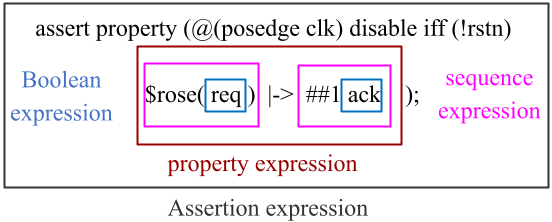
\includegraphics[width=0.65\linewidth]{Figs/FourLayersSVA.png}
    \caption{Four layers of an example concurrent assertion.}
    \label{fig:four-layers-sva}
\end{figure}
% In the following, an example concurrent assertion is shown:
% \begin{verbatim}
%     assert property (
%         @(posedge clk) disable iff (!rstn)
%         $rose(req) |-> ##1 ack
%     );   
% \end{verbatim}
% At the Boolean layer the only combinational expressions are the individual signals \texttt{req} and \texttt{ack}.
% At the sequence layer, there are two sequence expressions. The first is \texttt{\$rose(req)} and the second is \texttt{\#\#1} ack.
% In the Property layer, those two sequence expressions are combined by the operator \texttt{|->}, yielding the property expression \texttt{\$rose(req) |-> \#\#1 ack}. 
% In the context of \texttt{|->} and \texttt{|=>}, which are also called \textit{implication operator}s, their first operand is called \textit{precondition} and the second operand is called \textit{consequent}.
% Thus, \texttt{\$rose(req)} is the precondition and \texttt{\#\#1 ack} is the consequent.
% Finally, the verification layer binds the property expression to \texttt{@(posedge clk)} specifying the verification occuring on each rising edge of \texttt{clk}, and the clause disable \texttt{iff (!rstn)} specifying the verification occuring when \texttt{rstn} is $1$, which is futher wrapped by \texttt{assert property()}.
% The non-overlapping implication  $|$\verb|->| connects two parts:
% \begin{itemize}
%     \item the \textit{precondition}, \verb|req|, which specifies the event to monitor at the clock edge;
%     \item the \textit{consequent}, \verb|##1 ack|, which describes the expected behavior following the precondition. 
% \end{itemize}
% Specifically, this assertion specifies that when signal \verb|req| is true at a rising clock edge (precondition), then signal \verb|ack| must be true exactly one clock cycle later (consequent).
% In other words, the assertion does not evaluate the consequent if the precondition is never satisfied.
% % In other words, the assertion will not check the consequent when the precondition can never be true.
% This structure of a precondition and consequent also applies to the overlapping implication operator $|$\verb|=>|, although the timing behavior differs slightly.
\begin{table}[t]
\centering
\caption{Sequence SVA Operators}
\label{tab:sequence_sva_operators}
\begin{tabular}{|c|c|}
\hline
\textbf{SVA Operator} & \textbf{Explanation} \\ \hline
\texttt{\#\#N s} & \tabincell{l}{The evaluation of sequence expression \texttt{s} is delayed\\ by \texttt{N} clock cycles.} \\ \hline
\texttt{\$rose(s)} & \tabincell{l}{Returns $1$ if the LSB of sequence expression \texttt{s}\\ changed to $1$. Otherwise, returns $0$.} \\ \hline
\texttt{\$fell(s)} & \tabincell{l}{Returns $1$ if the LSB of sequence expression \texttt{s}\\ changed to $0$. Otherwise, returns $0$.} \\ \hline
\texttt{\$past(s,N)} & \tabincell{l}{Returns the value of sequence \texttt{s} in a \texttt{N} clock cycle \\step prior to the current one.} \\ \hline
\texttt{\$stable(s)} & \tabincell{l}{Returns $1$ if the value of sequence expression \texttt{s}\\ did not change. Otherwise, returns $0$.} \\ \hline
\texttt{\$onehot(s)} & \tabincell{l}{Returns $1$ if one bit of sequence expression \texttt{s}\\ is $1$. Otherwise, returns $0$.} \\ \hline
\texttt{\$onehot0(s)} & \tabincell{l}{Returns $1$ if no more than one bit of sequence\\ expression \texttt{s} is $1$. Otherwise, returns $0$.} \\ \hline
\end{tabular}
\end{table}

\begin{table}[t]
\centering
\caption{Property SVA Operators}
\label{tab:property_sva_operators}
\begin{tabular}{|c|c|}
\hline
\textbf{SVA Operator} & \textbf{Explanation} \\
\hline
\texttt{s |-> p} & \tabincell{l}{for every match of the sequence expression \texttt{s} \\beginning at the start point, the evaluation of\\ property expression \texttt{p} beginning in the current\\ clock cycle at the end point of the match \\succeeds and returns $1$.} \\ \hline
\texttt{s |=> p} & \tabincell{l}{for every match of the sequence expression \texttt{s} \\beginning at the start point, the evaluation of\\ property expression \texttt{p} beginning in the next\\ clock cycle at the end point of the match \\succeeds and returns $1$.} \\ \hline
\texttt{s\_eventually p} & \tabincell{l}{Return $1$ if there exists a current or future clock \\cycle at which property expression \texttt{p} is $1$.} \\ \hline
\end{tabular}
\end{table}

\subsection{Retrieval-Augmented Generation}
\label{subsec:RAG}
RAG is a technique that enhances the performance of LLMs by incorporating relevant external knowledge~\cite{Lewis20}.
%, especially on domain-specific tasks. 
Instead of relying solely on the LLM's internal knowledge, RAG augments the model’s input by retrieving relevant external documents from a knowledge database based on the query.
RAG has been successfully applied in different fields, such as code generation~\cite{Koziolek24}, medical QA~\cite{xiong2024}, financial QA~\cite{Setty24}, and conversational agents~\cite{alonso2024}.
% In Fig.~\ref{fig:Flow-of-Basic-RAG}, it shows the flow of basic RAG, which consists of two key components. 

RAG methods leverage a specialized database of \textit{vector embeddings}, created by first splitting the source materials, such as documents or code repositories, into smaller \textit{chunks} and then transforming each chunk into a numerical representation using an embedding model, i.e., a vector embedding. 
% By storing these embeddings as indexes in the database, the system can efficiently retrieve relevant information based on \textit{similarity search} when it receives a user’s input prompt.
The strategy used for splitting the source materials significantly impacts the relevance of retrieved chunks to the input prompt. 
A common practice is to apply \textit{static splitting}, where the source data is divided into fixed-size text chunks, typically based on a constant number of characters. 
A common method for enhancing the static splitting techniques is to employ LLM-based splitting, which leverages LLMs to identify more semantically coherent chunk boundaries~\cite{singh24,chang24n,dong24}.
However, they require careful prompt design and substantial computational overhead.
%While simple to implement, static splitting often ignores semantic boundaries in the content, separating logically related information across different chunks and thereby degrading retrieval quality.

The \textit{retrieval process}, which serves as the second key component of RAG, begins with an input prompt.
% As is shown in Fig.~\ref{fig:Flow-of-Basic-RAG}, the \textit{retrieval process}, which is the other key part of RAG, begins with an \textit{initial prompt}, which can be a question, an instruction, or another form of request for information. 
This prompt is transformed into a vector embedding using the same embedding model for constructing the database.
Then, the retrieval process uses \textit{similarity search} to identify the top-ranked or most similar chunks that align with the the input prompt, returning them as the \textit{relevant context}.
The original input prompt is then augmented with the relevant context to form a \textit{combined prompt}, enriching the LLM with domain-specific knowledge. 
The combined prompt guides the LLM to generate more accurate and context-aware responses. 
% RAG effectively bridges the gap between the model’s internal knowledge and the external information retrieved from the database, leading to informed and reliable results.

% The original prompt is then augmented with this retrieved context to form a \textit{combined promp}t, providing the LLM with direct, domain-specific information that may not be fully captured by its training alone.
% Finally, the combined prompt instructs the LLM to generate more accurate responses.

%The final generation step occurs when the LLM processes the combined prompt and produces a response. 
% Thus, RAG bridges the gap between the model’s internal knowledge, learned during pre-training, and the external knowledge retrieved in the database, leading to more informed and reliable results.

% \begin{figure}
%     \centering
%     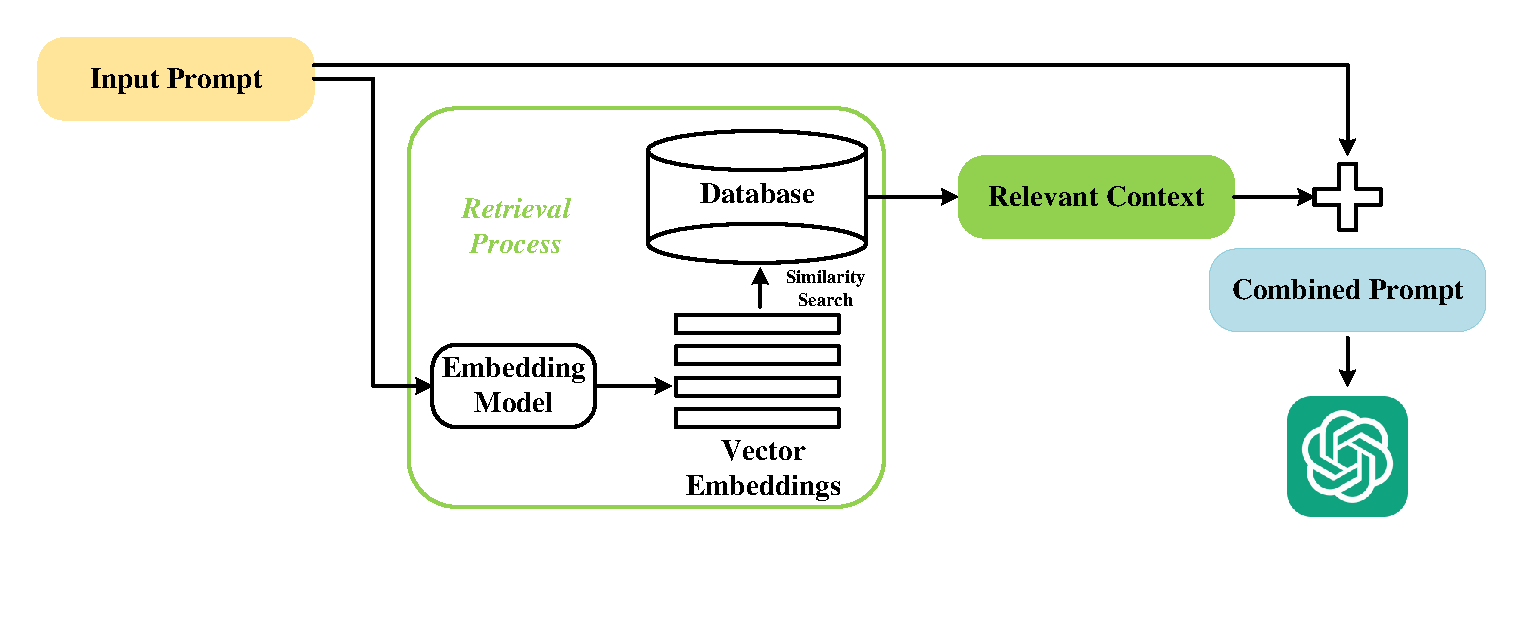
\includegraphics[width=\linewidth]{Figs/Basic_RAG_Flow.pdf}
%     \caption{Flow of basic RAG.}
%     \label{fig:Flow-of-Basic-RAG}
% \end{figure}

\subsection{Related Works}
A critical component for evaluating LLM-based
NL2SVA is the evaluation dataset. 
Prior works such as \textit{AssertionBench}~\cite{Vaishnavi25}, \textit{AssertLLM}~\cite{Yan25}, and \textit{FVEval}~\cite{Minwoo24} have provided open-source
datasets for benchmarking assertion generation. 
However, AssertionBench and AssertLLM lack detailed contextual information, such as natural language explanations of the SVAs.
This missing information is essential for rigorously evaluating
the functionality match between the generated SVAs and their
expected natural language property descriptions. 
FVEval introduces a more comprehensive dataset, containing $13$ hardware
designs, $80$ SVAs with corresponding human-written property
explanations.


\section{Methodology}
This section will introduce the main work of this paper.
In Section~\ref{subsec:RAGSVAG}, it introduces the proposed customized RAG framework for NL2SVA.
In Section~\ref{subsec:synthetic-finetuning-dataset}, it introduces the proposed fine-tuning dataset with prompt-guided explanations.
In Section~\ref{subsec:Evaluation-Dataset}, it introduces the proposed evaluation dataset.

\subsection{Customized RAG Framework for NL2SVA}
\label{subsec:RAGSVAG}
The overall flow is illustrated in Fig.~\ref{fig:overallflow-RAGSVAG}. 
% Starting from a given Verilog design and its corresponding assertion specification, the framework first utilizes a customized RAG pipeline to retrieve relevant contextual information with the input assertion specification. 
Given a Verilog design and a natural language assertion specification, the framework first applies a customized RAG to retrieve relevant contextual information based on the input specification.
The customized RAG component is built upon two key techniques: 
\textit{dynamic splitting} for constructing a code-based retrieval database from SystemVerilog textbooks (Section~\ref{subsubsec:Dynamic-Splitting}), and \textit{HybridRetrieval} that enhances the retrieval  by integrating global semantic retrieval with keyword-guided retrieval (Section~\ref{subsubsec:HybridRetrieval}). 
The retrieved information is incorporated into the \textit{Initial Input Prompt} to assist in generating a better initial SVA. 
The initial input prompt is shown in Fig.~\ref{fig:initial_sva_generation_prompt}.
\begin{figure}
    \centering
    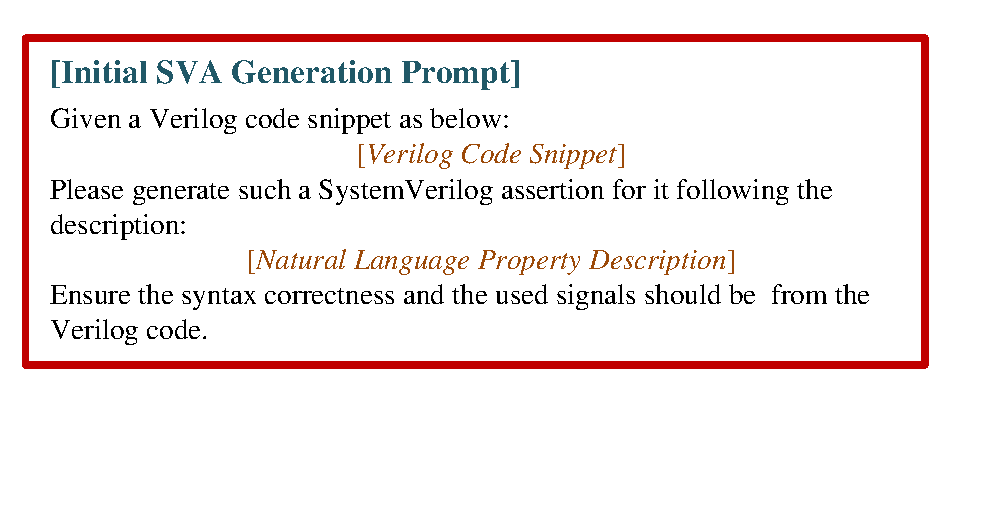
\includegraphics[width=\linewidth]{Figs/Initial-SVA-Generation.pdf}
    \caption{Initial SVA generation prompt.}
    \label{fig:initial_sva_generation_prompt}
\end{figure}
% \begin{framed}
% \begin{verbatim}
% // Initial SVA Generation Prompt
% Given a Verilog code snippet as below:
% ......

% Please generate such a systemverilog 
% assertion for it following the 
% description:
% ......

% Ensure the syntax correctness and the 
% used signals should be from the 
% verilog code.
% \end{verbatim}
% \end{framed}

To improve correctness of the generated assertion, an \textit{SVA operator-based rechecking} is applied (Section~\ref{subsubsec:SVA-Op-based-Rechecking}). 
This refinement step verifies and corrects the usage of SVA operators, ensuring better alignment between the generated assertion and the intended property description. 
Finally, it outputs a refined assertion.

\begin{figure}
    \centering
    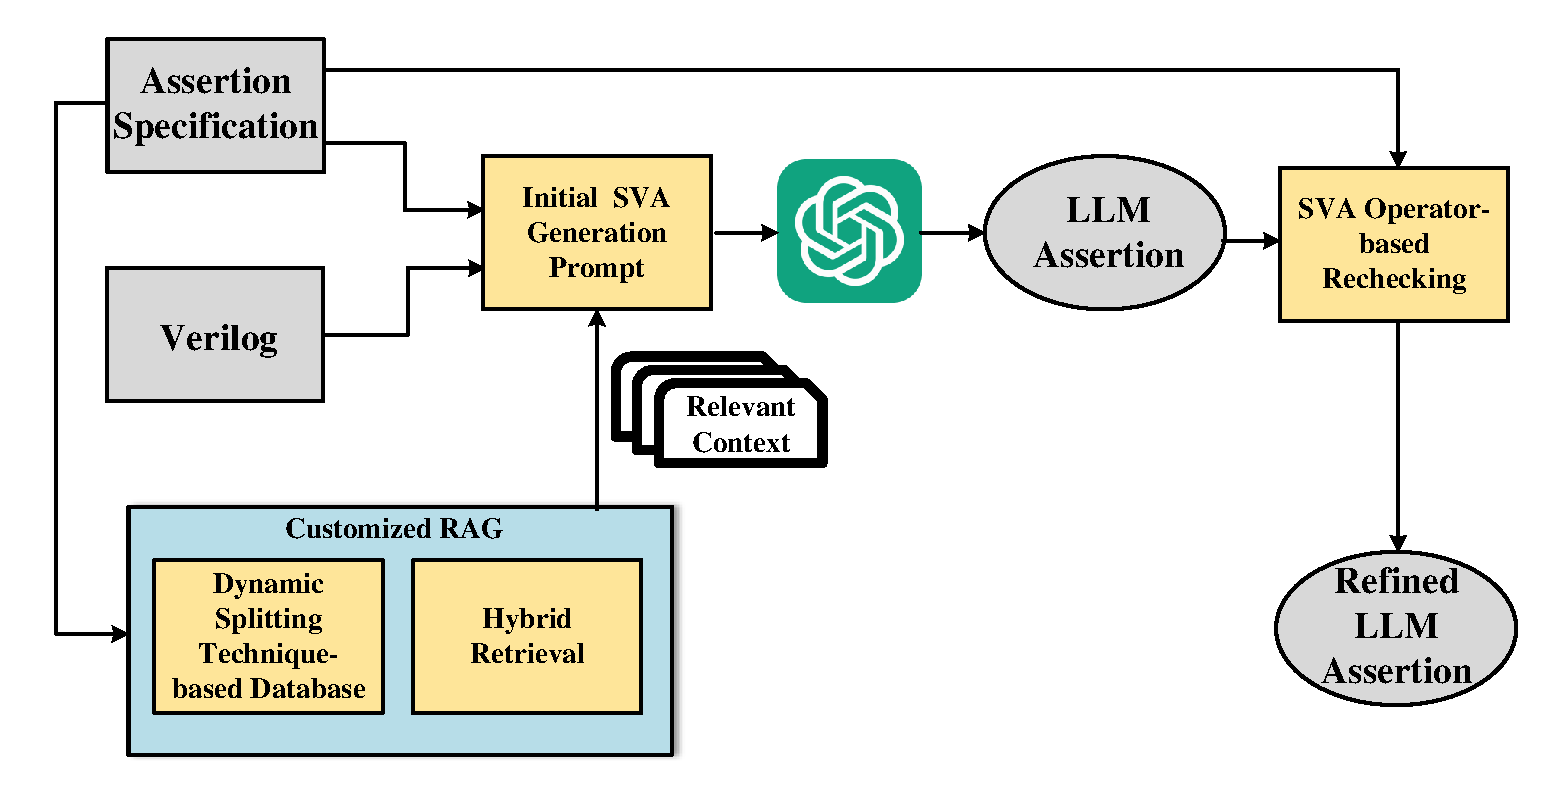
\includegraphics[width=\linewidth]{Figs/RAGSVAG.pdf}
    \caption{
    Overall flow of the proposed customized RAG framework: apply the proposed dynamic splitting to construct the database; apply the proposed HybridRetrieval to extract relevant context; apply the proposed SVA operator-based rechecking for correcting errors in generated SVAs.
    %Overall flow of the proposed RAGSVAG. {\bf Explain the flow here. You have two blocks with same name "Assertion Spec"  -->redraw to combine.}
    }
    \label{fig:overallflow-RAGSVAG}
\end{figure}
\subsubsection{Dynamic Splitting}
\label{subsubsec:Dynamic-Splitting}
addresses a key limitation of static splitting by distinguishing between code blocks and their related text. Instead of segmenting all content uniformly based on a fixed size threshold, our method constructs a specialized \textit{code database} designed to preserve the context surrounding each example.

The splitting process begins by parsing SystemVerilog textbooks to locate and isolate code snippets. 
% A \textit{font-based detection} is employed to recognize lines formatted in a distinctive style, such as a monospace font like \textit{Courier}. 
Whenever a code block is detected, the system automatically gathers the paragraph immediately preceding the code and the paragraph immediately following it. 
These three elements, consisting of the paragraph before, the code snippet itself, and the paragraph after, are combined into a single chunk, called \textit{code-centric chunk}. 
% This packaging ensures that the code snippet and its surrounding context, which is highly likely to be relevant to the code or its explanation, are preserved together within the same retrieval chunk.
% By packaging the code snippet together with its surrounding paragraphs, the local context that describes or references the code is preserved within the same retrieval unit.
Code-centric chunks are retained to construct the code database. 
Paragraphs not adjacent to a code snippet are not separately stored. 
% During retrieval, the system queries this code database to obtain relevant code examples along with their immediate natural language explanations.
By splitting content in this semantically-aware manner and focusing retrieval on code-centric contexts, dynamic splitting improves the relevance and precision of retrieved knowledge.
\subsubsection{HybridRetrieval}
\label{subsubsec:HybridRetrieval}
In addition to limitations in database construction, the retrieval process itself presents significant challenges when applying the basic RAG framework to SVA generation. Standard retrieval mechanisms based on global semantic similarity of the input prompt fail to capture fine-grained semantic embedded in natural language property specifications. Temporal relationships and operator-specific behaviors may be overlooked, resulting in the retrieval of incomplete or irrelevant contexts.

To address this issue, we propose \textit{HybridRetrieval}, a two-path retrieval mechanism that enhances context relevance by combining global semantic retrieval with keyword-guided operator retrieval. The overall flow is illustrated in Fig.~\ref{fig:HybridRetrieval}.
Given a natural language assertion specification, HybridRetrieval initiates two retrieval paths in parallel.
\begin{itemize}
    \item In the first path, a standard basic RAG retrieval is performed by embedding the entire input specification and retrieving chunks from the constructed code database based on global semantic similarity. 
    This step captures relevant contextual information corresponding to the global semantic of the property description.
    \item In the second path, the LLM is sequentially instructed with two custom prompts to extract fine-grain operator-related context. 
\end{itemize}
\begin{figure}
    \centering
    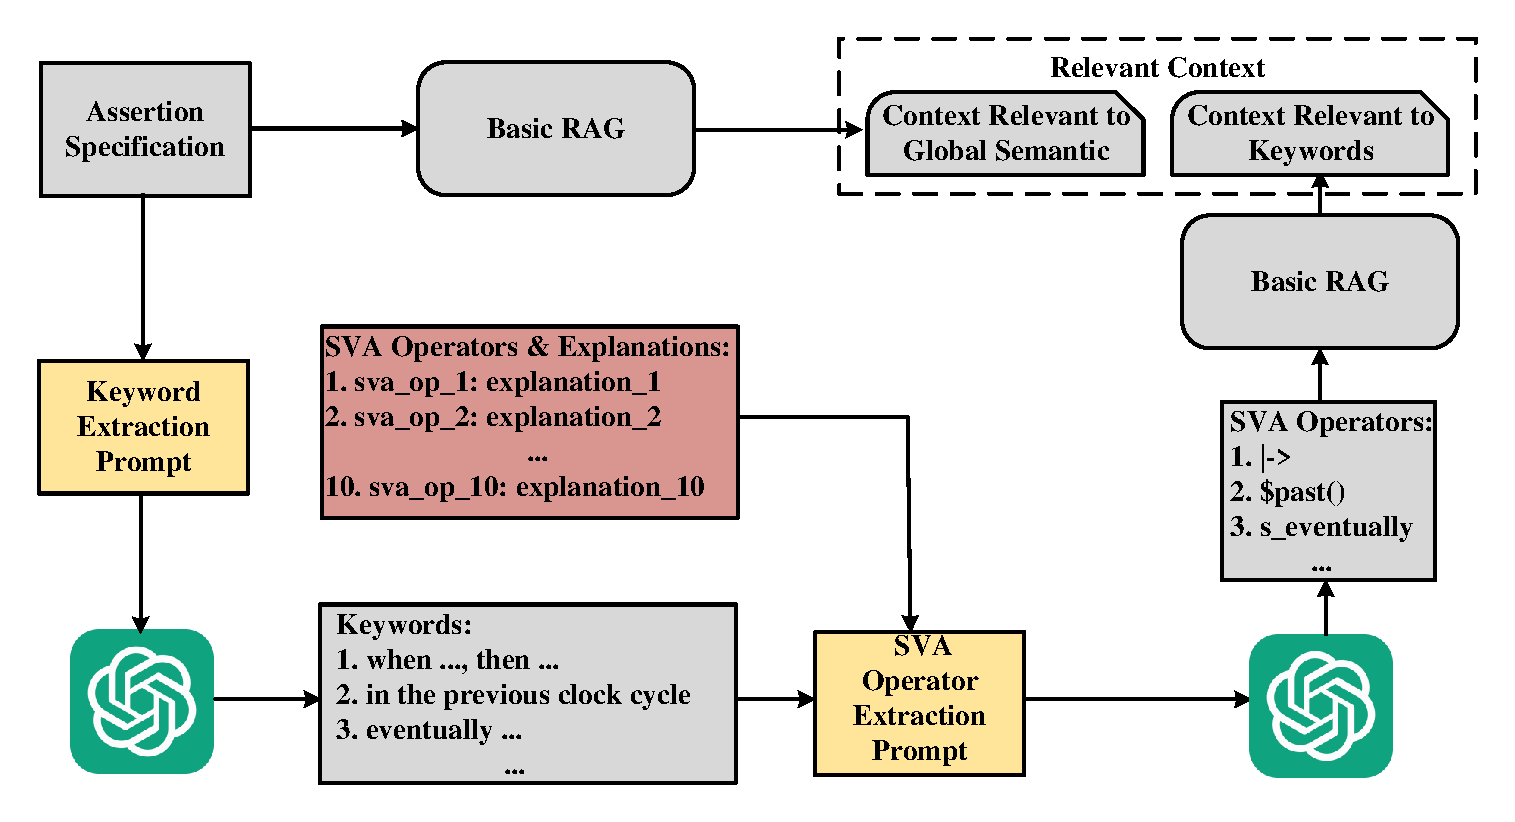
\includegraphics[width=\linewidth]{Figs/HybridRetrieval.pdf}
    \caption{Flow of HybridRetrieval combines the global semantic retrieval and the keyword-guided operator retrieval.}
    \label{fig:HybridRetrieval}
\end{figure}

The first prompt is the \textit{Keyword Extraction Prompt}. 
It instructs the LLM to decompose the natural language description of the assertion into multiple parts, each representing an operation over a single signal or a group of signals.
Examples of such keywords include phrases like \texttt{in the previous clock cycle}, which indicate the presence of temporal relationships between signals.
The keyword extraction prompt is shown in Fig.~\ref{fig:keyword_extraction_prompt}.
\begin{figure}
    \centering
    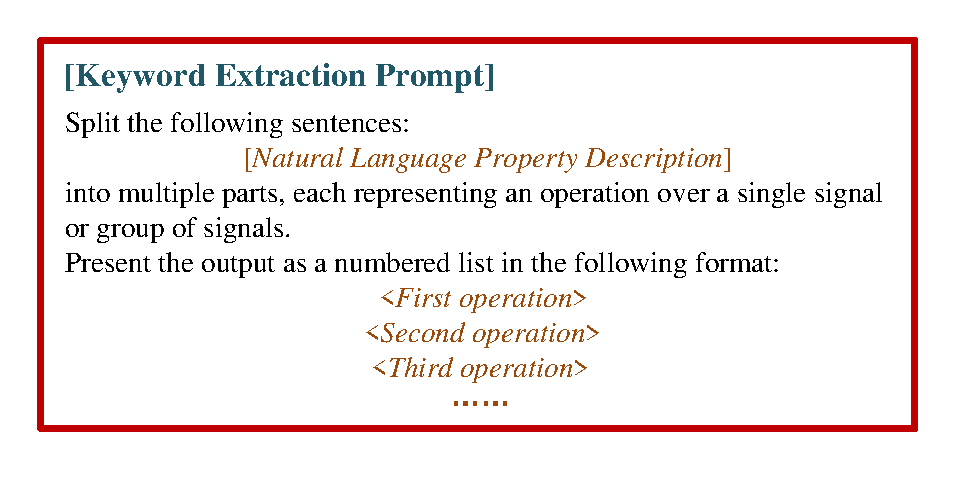
\includegraphics[width=\linewidth]{Figs/Keyword-Extraction.pdf}
    \caption{Keyword extraction prompt.}
    \label{fig:keyword_extraction_prompt}
\end{figure}
% \begin{framed}
% \begin{verbatim}
% // Keyword Extraction Prompt
% Split the following sentence: 
% ...... 

% into multiple parts, each representing 
% an operation over a single signal or 
% group of signals. 

% Present the output as a numbered list 
% in the following format:

% <First operation>
% <Second operation>
% <Third operation>
% ......
% \end{verbatim}
% \end{framed}

The second prompt is the \textit{SVA Operator Extraction Prompt}, which is then used to instruct LLM to map each extracted keyword to the most relevant SVA operator.
% To control the complexity and accuracy of mapping process, we construct a \textit{SVA Quick Reference Table} and instruct the LLM to map the most relevant operator from it.
To balance the complexity and accuracy of the mapping process, we prompt the LLM to select the most relevant operator from the $10$ SVA operators shown in Table~\ref{tab:sequence_sva_operators} and Table~\ref{tab:property_sva_operators}.
% To balance the complexity and accuracy of the mapping process, we construct an \textit{SVA Quick Reference Table}, consisting of a set of SVA operators and their corresponding natural language explanations, and prompt the LLM to select the most relevant operator from it.
% The SVA quick reference table is constructed by selecting ten commonly used SVA temporal operators, shown in Table~\ref{tab:sva_operators}.
% by referencing our constructed SVA quick reference table in Table~\ref{tab:sva_operators}. 
% The SVA quick reference table is constructed by selecting the ten commonly used SVA temporal operators.
The SVA operator extraction prompt is shown in Fig.~\ref{fig:sva_operators_extraction_prompt}.
\begin{figure}
    \centering
    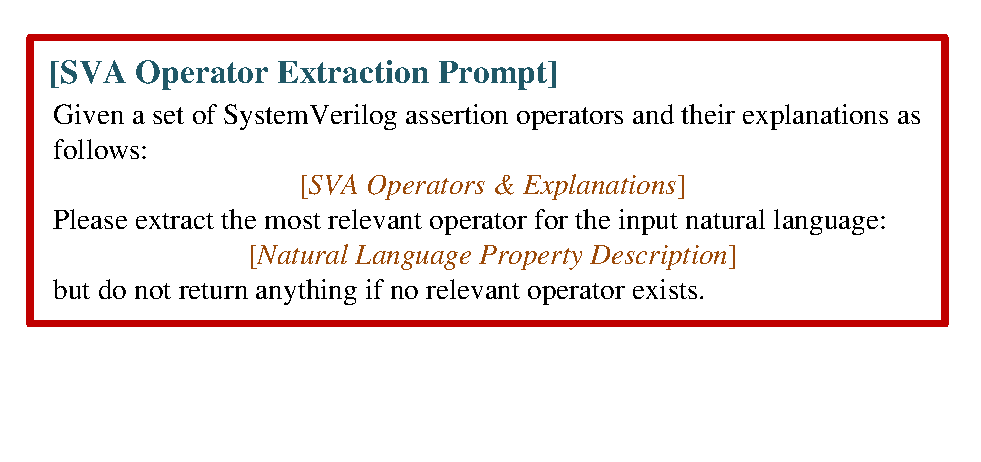
\includegraphics[width=\linewidth]{Figs/SVA-Operator-Extraction.pdf}
    \caption{SVA operators extraction prompt.}
    \label{fig:sva_operators_extraction_prompt}
\end{figure}
% \begin{framed}
% \begin{verbatim}
% // SVA Operator Extraction Prompt
% Given a set of SystemVerilog assertion 
% operators and their explanations as 
% follows: 
% ......

% Please extract the most relevant 
% operator for the input natural 
% language:
% ......

% but do not return anything if no 
% relevant operator exists.
% \end{verbatim}
% \end{framed}

Once the relevant SVA operators are identified, a RAG retrieval is conducted. 
This retrieval  targets database chunks that mention or explain the identified operators, ensuring that the retrieved context is not only semantically relevant but also aligned with the SVA operator semantics necessary for correct assertion construction.

Finally, the outputs from the global semantic and the operator-guided retrievals are combined with the initial SVA generation prompt to enrich the prompt. 
By integrating both the property semantics and operator-specific contexts, HybridRetrieval can improve the quality and completeness of information for the LLM during SVA generation.

% In addition to limitations in database construction, the retrieval process itself presents significant challenges when applying basic RAG frameworks to SVA generation. Standard retrieval mechanisms based purely on global semantic similarity often fail to capture fine-grained cues embedded in natural language property specifications. 
% Specifically, temporal relationships and operator-specific behaviors may be overlooked, leading to the retrieval of incomplete or irrelevant contexts.

% To address this limitation, we propose HybridRetrieval, which integrates global semantic retrieval with keyword-guided retrieval to enhance the specificity of retrieved knowledge. 
% As illustrated in Fig.~\ref{fig:HybridRetrieval}, the retrieval process begins with an initial prompt that describes a natural language property. 
% A global semantic retrieval first selects database chunks that are broadly related to the meaning of the prompt based on embedding similarity, which is just the same as the retrieval in basic RAG.

% Simultaneously, a keyword extraction stage is initiated. Using a lightweight LLM prompt, critical temporal or behavioral keywords are extracted from the input description. Examples of such keywords include phrases like "when..., then..." or "in the previous clock cycle," which suggest the presence of temporal dependencies. 
% These extracted keywords are then mapped to corresponding SystemVerilog operators, such as $|$\verb|->|, \verb|$past()|, or \verb|s_eventually|, using a curated operator reference table.
% This mapping process

% A second retrieval pass focuses specifically on locating database chunks that mention the identified SVA operators. By combining the results of both the global semantic search and the operator-guided search, HybridRetrieval forms an enriched set of contexts. This hybrid strategy ensures that the retrieved material captures both the overall semantic meaning of the input property and the specific temporal constructs critical for generating accurate SystemVerilog Assertions.


% \begin{table}[t]
% \centering
% \caption{SVA Quick Reference Table in RAGSVAG}
% \label{tab:sva_operators}
% \begin{tabular}{|c|c|}
% \hline
% \textbf{SVA Operator} & \textbf{Explanation} \\ \hline
% \texttt{\$rose} & \tabincell{l}{Detects that the condition transitions from false to \\true (rising edge).} \\ \hline
% \texttt{\#\#$n$} & \tabincell{l}{Delay operator that postpones evaluation by $n$ \\clock cycle.} \\ \hline
% \texttt{\$stable} & \tabincell{l}{Ensures that the signal value remains unchanged\\ during the evaluation cycle.} \\ \hline
% \texttt{|->} & \tabincell{l}{Overlapping implication operator, meaning that\\ if the conditions on the left are met, the condition\\ on the right must hold in the same clock cycle.} \\ \hline
% \texttt{\$isunknown} & Checks if a signal has an unknown (X or Z) value. \\ \hline
% \texttt{s\_eventually} & \tabincell{l}{Temporal operator indicating that the contained\\ condition is required to occur at some future\\ clock cycle.} \\ \hline
% \texttt{\$onehot0} & \tabincell{l}{Function that checks that no more than one bit\\ of the operand is set to 1.} \\ \hline
% \texttt{|=>} & \tabincell{l}{Non-overlapping implication operator, meaning \\that if the conditions on the left are met, the \\condition on the right must hold in the next\\ clock cycle.} \\ \hline
% \texttt{\$onehot} & \tabincell{l}{Function that verifies that exactly one bit in the \\operand is set to 1.} \\ \hline
% \texttt{\$past} & Refers to the value from previous clock cycle(s). \\ \hline
% \end{tabular}
% \end{table}

\subsubsection{SVA Operator-based Rechecking}
\label{subsubsec:SVA-Op-based-Rechecking}
Even with the improved retrieval through HybridRetrieval, LLMs may generate assertions that misuse SVA operators. 
Misinterpretations occur because retrieved materials, although relevant, may contain both helpful and noisy information. 
Certain SVA operators exhibit slight semantic differences, such as \texttt{|->} and \texttt{|=>}, that are difficult for LLMs to distinguish during initial generation, particularly regarding precise timing and logical behavior.

To address these challenges, we propose an SVA operator-based rechecking flow. 
% Given a LLM generated assertion, a rechecking stage is introduced to check the functional correctness of the generated assertion with respect to the original natural language property description.
In this stage, the flow first extracts the list of operators present in the generated assertion. 
The relevant explanations for these operators are then retrieved from Table ~\ref{tab:sequence_sva_operators} and Table~\ref{tab:property_sva_operators}. 
Given these context, the \textit{SVA Rechecking Prompt} is applied to instruct the LLM to verify the correct use of SVA operators in the LLM-generated assertion. 
The SVA rechecking prompt is shown in Fig.~\ref{fig:SVA_Checking_Prompt}.
\begin{figure}
    \centering
    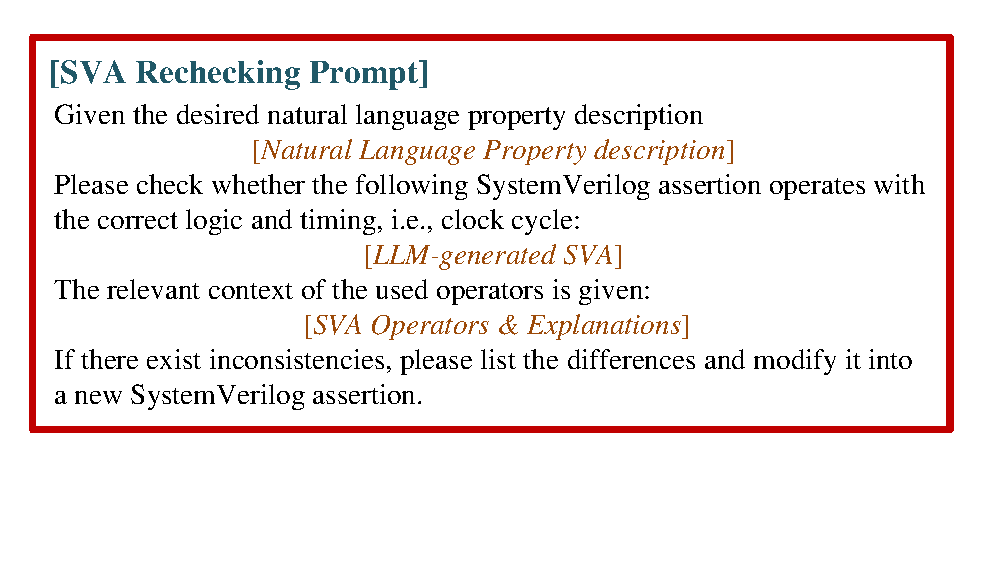
\includegraphics[width=\linewidth]{Figs/SVA-Rechecking.pdf}
    \caption{SVA checking prompt.}
    \label{fig:SVA_Checking_Prompt}
\end{figure}
% \begin{framed}
% \begin{verbatim}
% // SVA Rechecking Prompt
% Given the desired natural language 
% property description 
% ......

% Please check whether the SystemVerilog 
% assertion 
% ......

% operates with the correct logic and 
% timing (i.e., clock cycle).

% The relevant context of the used 
% operators is given: 
% ...... 

% If there exist inconsistencies, please 
% list the differences and modify it 
% into a new SystemVerilog assertion.
% \end{verbatim}
% \end{framed}

% By incorporating the operator-based rechecking flow, the framework enhances the correctness of SVA operator usage and improves the overall quality of LLM-generated assertions.

% Even with improved retrieval through HybridRetrieval, LLMs may still generate assertions that misuse SystemVerilog operators. Misinterpretations often occur because retrieved materials, although relevant, may contain both helpful and noisy information. Additionally, certain SVA operators exhibit subtle semantic differences that are difficult for LLMs to distinguish during initial generation.

% To further improve the functional correctness of generated assertions, we propose an SVA operator-based rechecking flow, as illustrated in Fig. 2. After the LLM generates an initial assertion, the system first extracts the list of SVA operators present in the assertion text. Each extracted operator is cross-checked against an SVA operator reference, which provides a concise description of its intended behavior and temporal semantics.

% A rechecking prompt is then constructed, incorporating both the original natural language description and the generated assertion. The LLM is tasked with verifying whether the assertion correctly reflects the intended functionality of the identified operators. If inconsistencies or mismatches are found between the operator semantics and the assertion behavior, the LLM is instructed to revise and correct the assertion accordingly.

% This operator-based rechecking flow serves as a post-generation refinement step that ensures not only syntactic correctness but also deeper semantic alignment between the natural language property description and the formal SVA expression.
% \begin{figure}
%     \centering
%     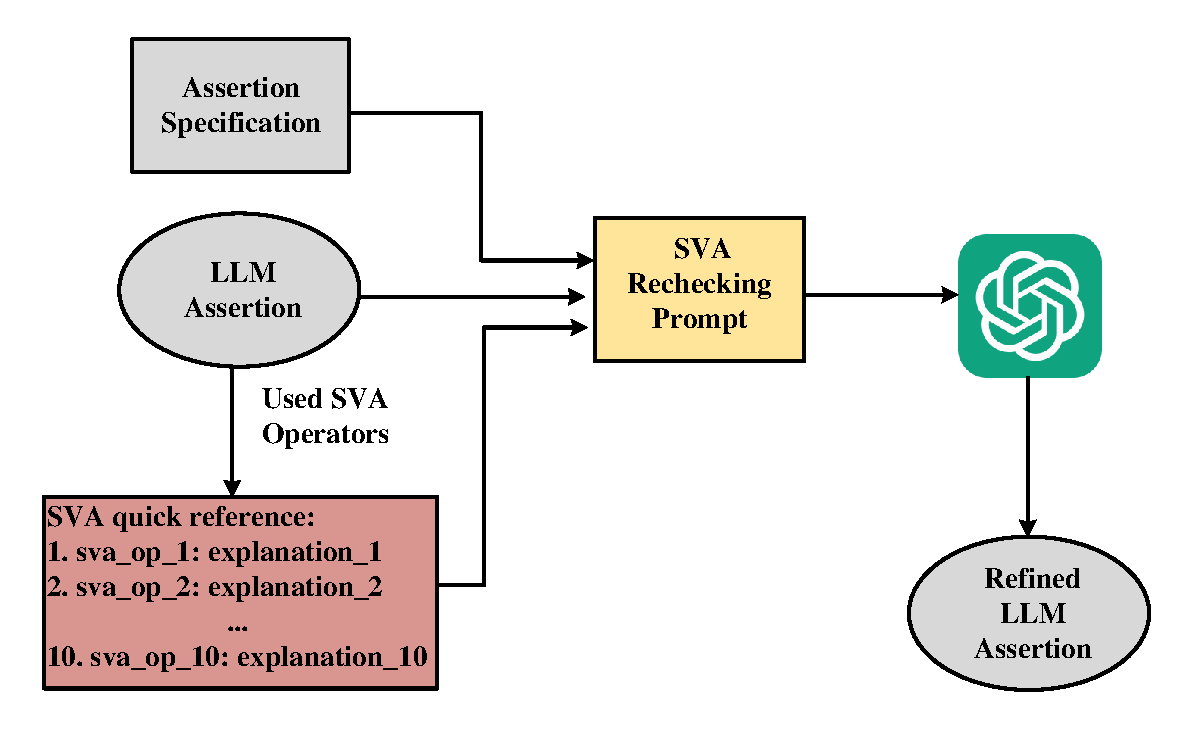
\includegraphics[width=\linewidth]{Figs/SVAOperatorRefine.pdf}
%     \caption{Flow of SVA operator-based rechecking.}
%     \label{fig:SVA-Rechecking}
% \end{figure}
\subsection{Synthetic Finetuning Dataset for NL2SVA}
\label{subsec:synthetic-finetuning-dataset}
Although Section ~\ref{subsec:RAGSVAG} introduces a customized RAG framework for guiding LLMs to do NL2SVA, lightweight LLMs may struggle to follow the different chained prompts in that pipeline. 
Their shorter context windows can also truncate the combined prompt and retrieved context, leading to incomplete or incoherent output. 
To overcome these limits, we prepare a supervised fine-tuning dataset that teaches smaller models to perform the NL2SVA task directly, without relying on long, multi-stage prompts.

By scraping Verilog codes from $67$ hardware-design textbooks spanning digital logic, computer architecture, SoC implementation, and formal verification, and extracting every embedded SVA, we obtained $4070$ ground-truth assertions.
Each assertion is paired with a concise, one-sentence natural language explanation produced by prompting \textit{OpenAI o4-mini} with the raw SVA and natural language explanations of SVA operators (Table~\ref{tab:sequence_sva_operators} and Table~\ref{tab:property_sva_operators}).
% For every assertion we then obtain a concise, one-sentence English description. \textit{OpenAI o4-mini} model receives the raw SVA together with a short glossary of SVA operators (Table 1) and is instructed to return a single behavioural statement. Because the prompt enforces length and style constraints, the resulting explanations are uniform and fit well within the context window of lightweight models.

The core feature of our fine-tuning dataset is a complete layer-by-layer derivation trace of each SVA from its corresponding natural language explanation. 
We refer to this trace as a \textit{Prompt-guided Explanation}. 
Section~\ref{subsec:SVA} describes the four layers of a concurrent SVA, and the prompt-guided explanation records how those layers are actually constructed for each individual case. 
The prompt-guided explanation is produced by OpenAI o4-mini. We feed each pair of the SVA and explanation to the LLM and instruct it to reconstruct the SVA from the explanation step by step as follows:
\begin{itemize}
    \item [(1)] Identify the top-level property SVA operator.
    \item [(2)] Split the natural language explanation into operand fragments that match the number of operands of the selected operator;
    \item [(3)] For each fragment, decide whether it represents a sequence or a property. If it is a sequence, translate it into a sequence expression directly; otherwise, recursively apply Steps $1$--$4$.
    \item [(4)] Combine the fragment expressions into the complete property expression using the selected property SVA operator.
    \item [(5)] Wrap the property expression in \texttt{assert property (...)}.
\end{itemize}
The detailed prompt for generating the prompt-guided explanation is shown in Appendix~\ref{subsec:prompt-guided-explanation-generation} and an example prompt-guided explanation is shown in Appendix~\ref{subsec:example-prompt-guided-explanation}.
\subsection{Evaluation Dataset}\label{subsec:Evaluation-Dataset}
In constructing our evaluation dataset, we aim to ensure both realism and quality in the SVAs. 
To achieve this, we gather $40$ Verilog designs and $229$ concurrent SVAs from a combination of open-source cores and academic verification courses. 
In Fig.~\ref{fig:sva-ops-signals}, it summarizes the operator and signal counts for all $229$ SVAs, showing the complexity of each SVA and indicating that most of them are non-trivial.

Each of them is verified to ensure syntax and functionality correctness using FPV tool \textit{Cadence JasperGold}~\cite{cadencejaspergold}. 
The evaluation dataset provides the  natural language property for each SVA, which is generated manually.
Note that each explanation does not contain any detailed signals, which are translated as natural language descriptions.
In Appendix~\ref{subsec:Example-SVAs}, it shows $10$ example natural language properties from our evaluation dataset. 
\begin{figure}
    \centering
    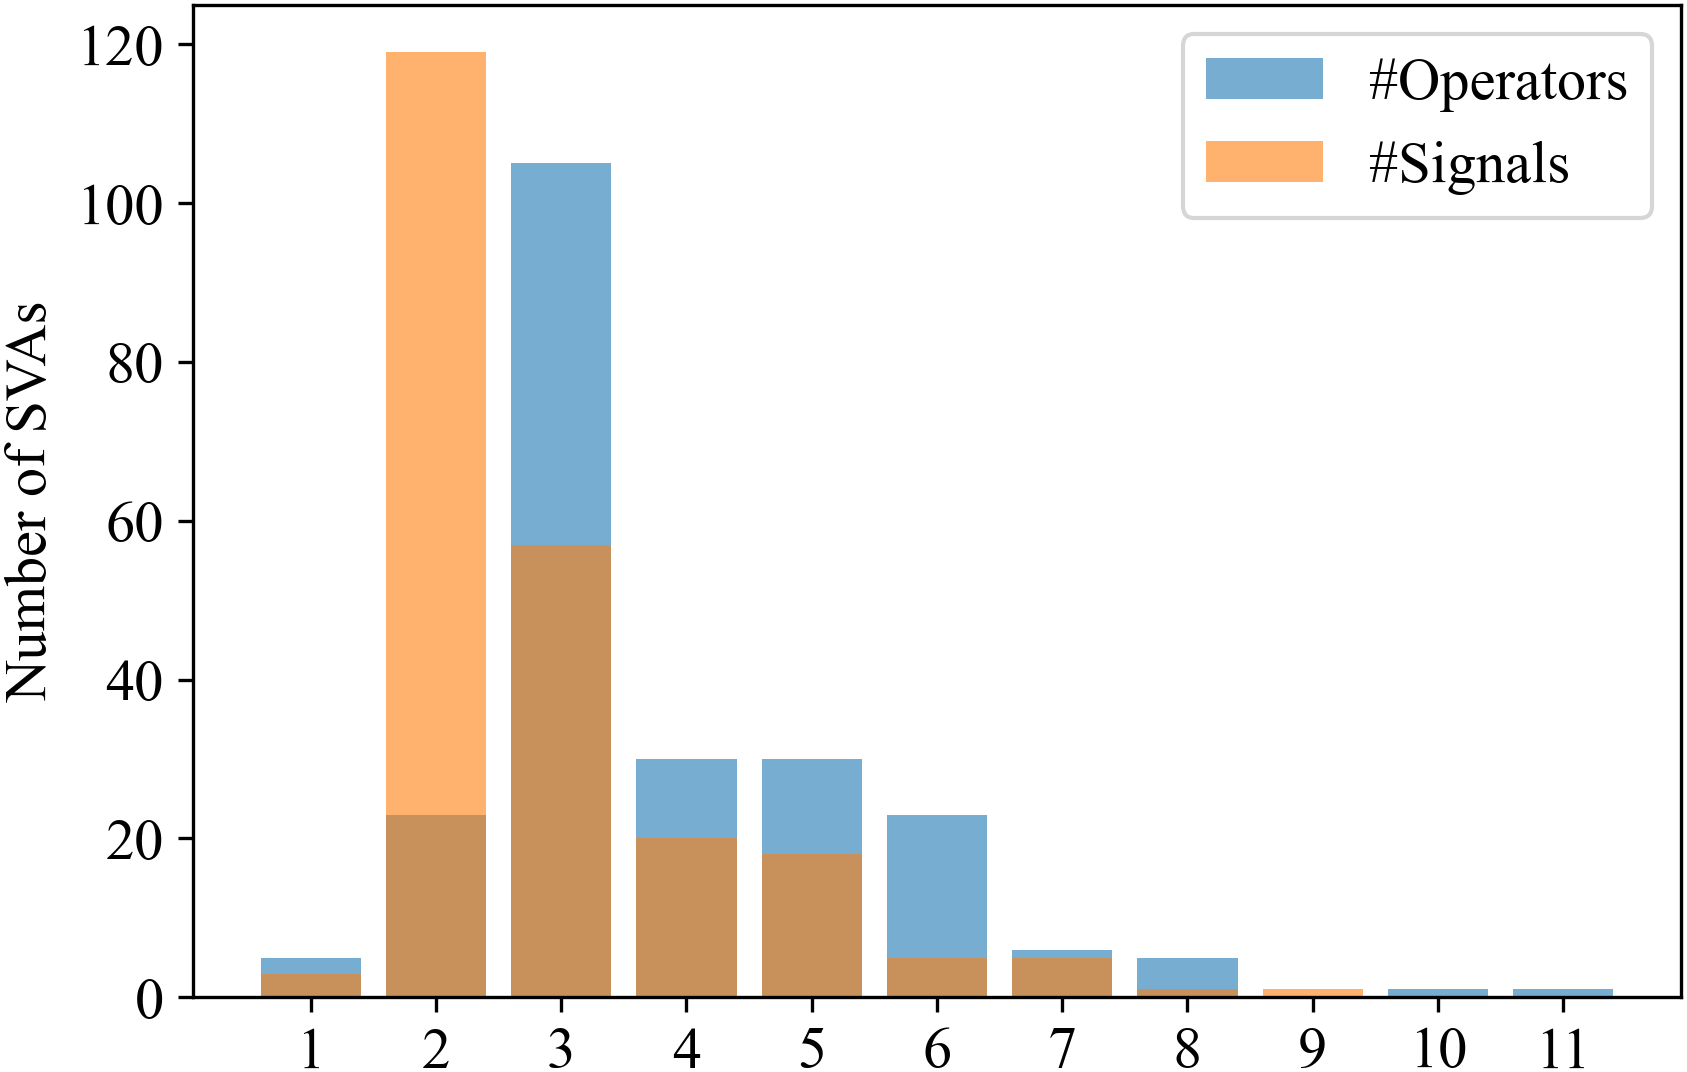
\includegraphics[width=0.9\linewidth]{Figs/op_signal_statistics.png}
    \caption{Number of SVA operators and signals in the $229$ SVAs.}
    \label{fig:sva-ops-signals}
\end{figure}
% These assertions are then subjected to a three-step validation process using the \textit{formal property verification} (\textit{FPV}) tool \textit{Cadence JasperGold}~\cite{cadencejaspergold}. 
% First, we check syntax correctness to confirm that each assertion is syntactically valid and could be parsed by the tool. 
% Second, we verify functionality correctness by running formal proofs on the designs and their corresponding assertions, ensuring that no counterexamples are generated.
% % Second, we test functionality correctness by running formal proofs on the designs and each assertion; no counterexamples are allowed to exist. 
% Some assertions use implication operators, which do not check properties unless the precondition is met as mentioned in Section~\ref{subsec:SVA}. 
% If there is no scenario that triggers the precondition, the assertion becomes meaningless. Third, in such situations, we examine whether the preconditions can be covered.
% Some assertions employ the implication operators. 
% As is mentioned in Section~\ref{subsec:SVA}, they will not check any properties when the precondition is not asserted.
% Thus, if there exists no case making the precondition assert, the assertion is meaningless.
% Third, in these cases, we check whether the preconditions can be covered.

% For each of the $40$ designs, we provide:
% \begin{itemize}
%     \item \textit{Verilog source code}: Verilog files that contain the RTL implementation of the design.
%     \item \textit{JSON file} that details each of the associated SVA:
%     \begin{itemize}
%         \item \textit{clock signal condition}
%         \item \textit{disable condition}
%         \item \textit{logical expression}
%         \item \textit{Signals}: a list of signals referenced by the assertion;
%         \item \textit{Assertion Explanation}: human-written explanation of the logic expression.
%     \end{itemize}
% \end{itemize}

% In Fig.~\ref{fig:example-evaluation-dataset}, it shows an example design \verb|register| and its associated JSON file from our evaluation dataset.
% The design has two associated SVAs, which can be extracted from the JSON file. 
% For example, the first assertion is 
% \begin{verbatim}
% assert property (@(posedge clk) 
%                  disable iff (rst) 
%                  en |=> out==$past(in,1));
% \end{verbatim}
% with the used signals \texttt{en}, \texttt{out}, \texttt{in}, and the human-written explanation: when enable signal is set (1), output 
% signal equals the last one clock cycle's 
% input signal from the next clock cycle.
% \begin{figure}
%     \centering
%     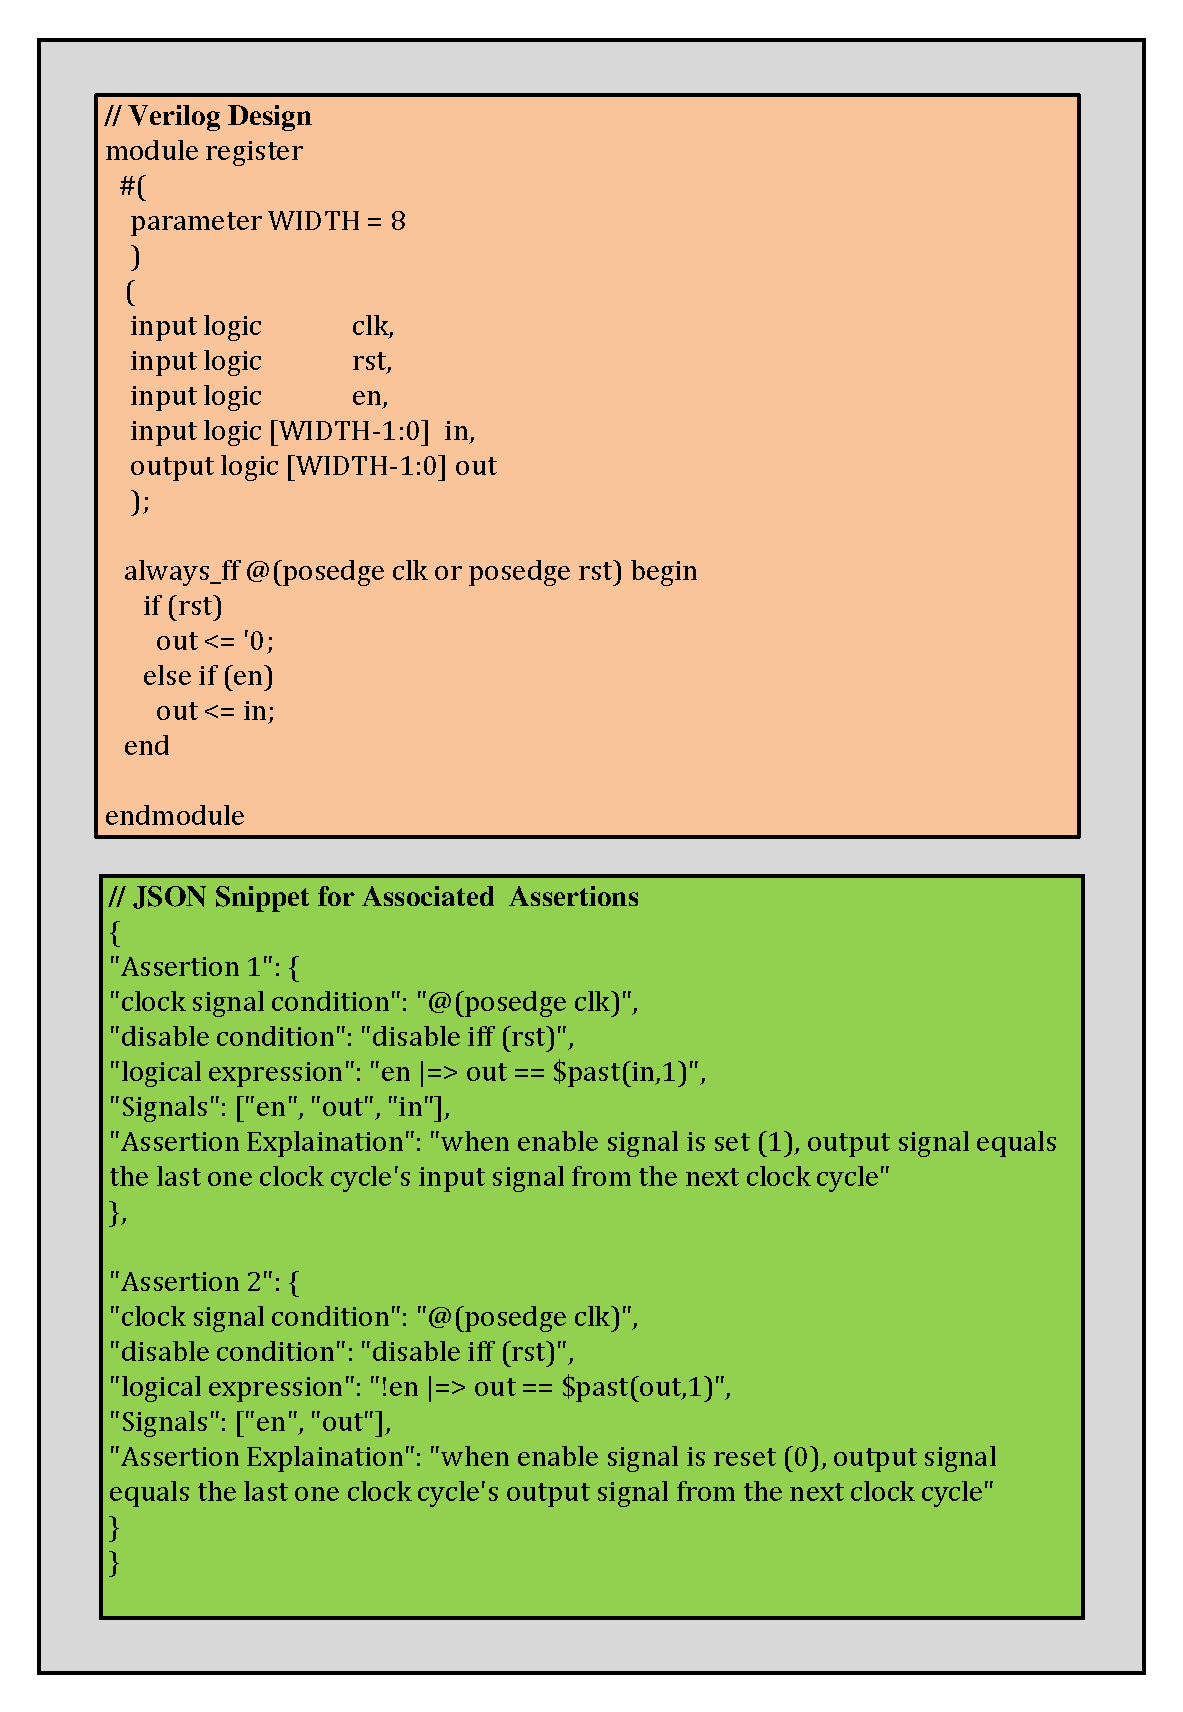
\includegraphics[width=1\linewidth]{Figs/Evaluation_Dataset.pdf}
%     \caption{An example Verilog design and the associated JSON file storing two SVAs and their corresponding details.}
%     \label{fig:example-evaluation-dataset}
% \end{figure}
% Implementation details
% are available in our repository\footnote{ https://github.com/FCHXWH823/RAG-aided-Assertion-Generation}.

% \begin{figure}
%     \centering
%     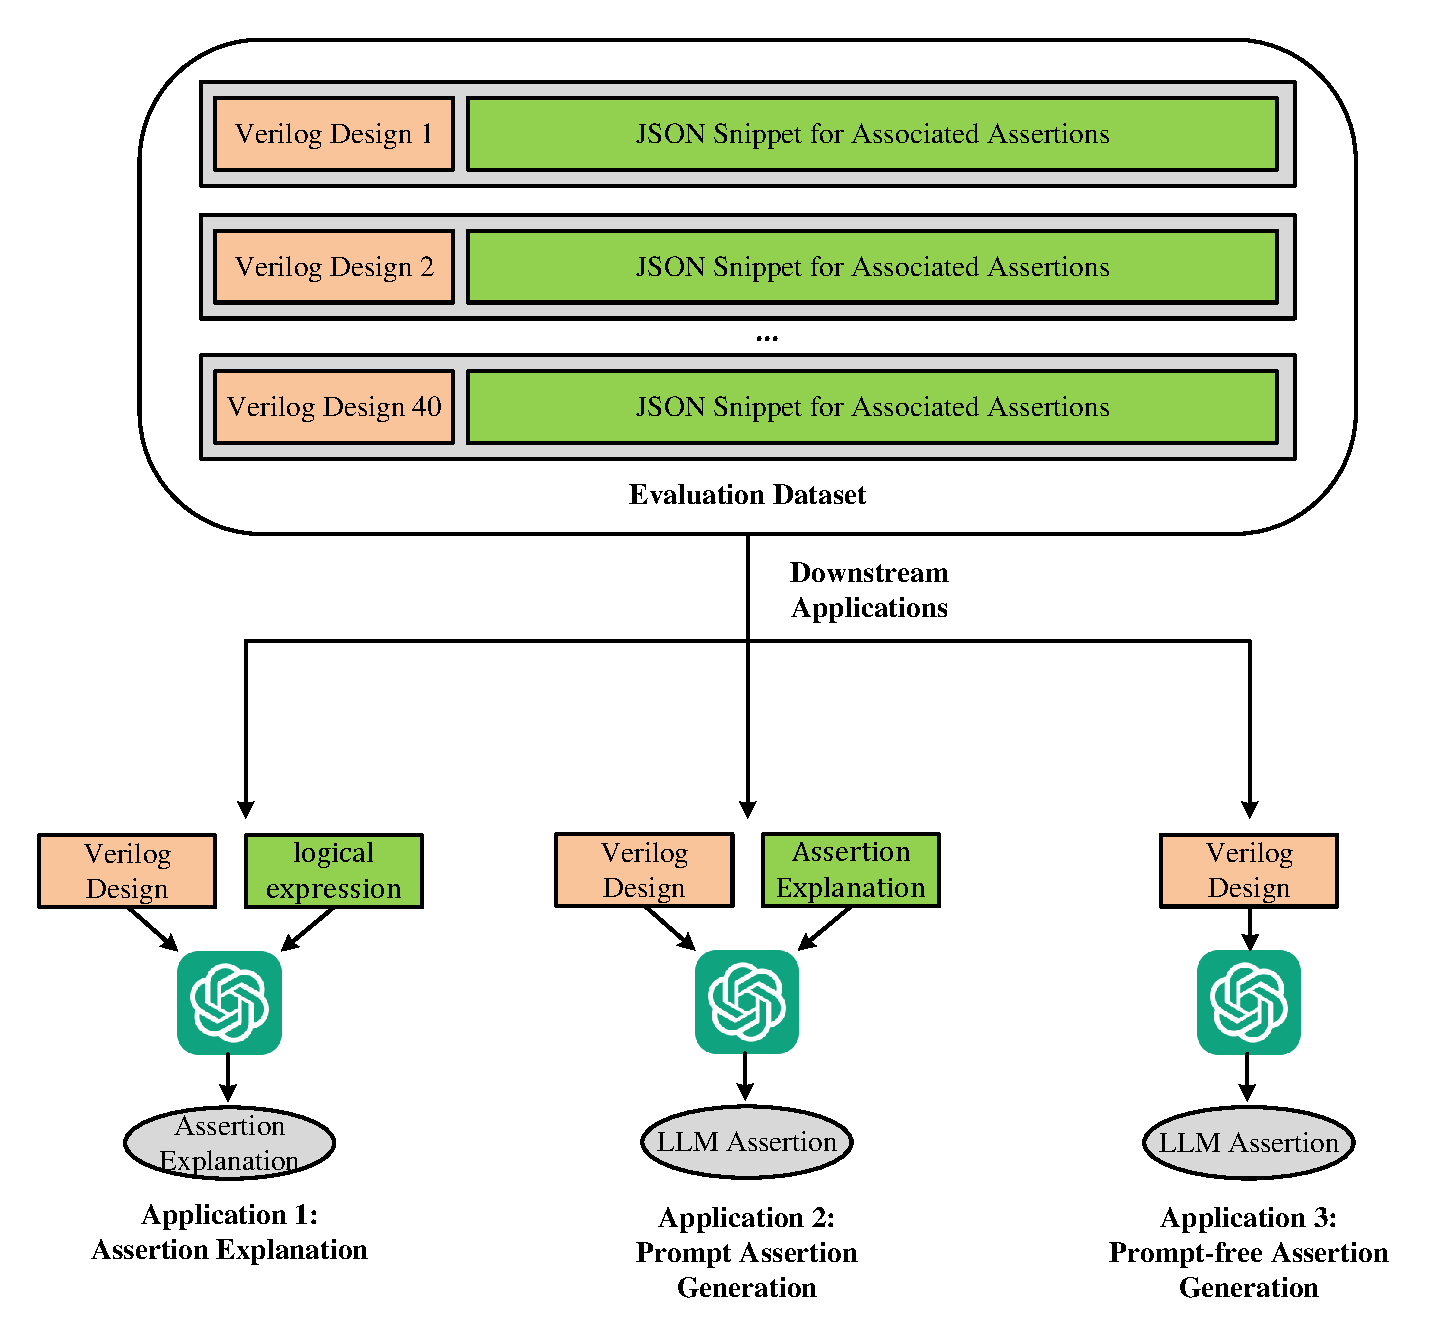
\includegraphics[width=\linewidth]{Figs/RAG_Downstream_Applications.pdf}
%     \caption{Support evaluating multiple downstream assertion-related tasks by the proposed evaluation dataset.}
%     \label{fig:down-stream-related-tasks}
% \end{figure}

% In Fig.~\ref{fig:down-stream-related-tasks}, our evaluation dataset supports assessing three different downstream assertion-related tasks because each assertion includes detailed annotations. 
% \begin{itemize}
%     \item \textit{Assertion Explanation}: In this task, the LLM is given an existing assertion along with the corresponding Verilog design context. 
%     The goal is to produce a human-readable explanation of what the assertion does.
%     This tests the LLM’s ability to interpret SystemVerilog syntax, understand the design’s functionality, and explain the purpose of a given property.
%     \item \textit{Prompt Assertion Generation}: the LLM is prompted with a natural language description of a property or behavior, along with relevant design context. 
%     The model must then generate the corresponding SVA. 
%     This scenario evaluates the LLM’s ability to map a natural language specification to the correct signals and syntaxes within an SVA, ensuring that the final assertion accurately captures the intended behavior.

%     \item \textit{Prompt-free Assertion Generation}:
%     the LLM receives only the Verilog design. 
%     It must output a meaningful set of assertions. 
%     This challenges the model to identify important design behaviors or corner cases on its own and encode them as SVAs. Evaluating performance on this task reveals how well the LLM can detect and formalize key properties from a design without explicit guidance.
%     \end{itemize}

% LLM-aided assertion generation is inherently challenging because it demands several distinct abilities.
% Our evaluation dataset enables a comprehensive evaluation of these different LLM abilities.
% This level of granularity is crucial for diagnosing which aspects of the LLM’s understanding or generation capabilities need further refinement, ultimately guiding targeted improvements in LLM-based assertion generation.

% Finally, an automatic evaluation framework is proposed to evaluate the effectiveness of our RAGSVAG.
% The pipeline begins with two key inputs: the Verilog design and its assertion specification, which are both from the evaluation dataset. 
% Then, our RAGSVAG receives the two inputs and outputs the corresponding SVA.
% % The two inputs are combined with the output assertion format to construct the \textit{initial prompt}. 
% % The template of the initial prompt is shown in Fig.~\ref{fig:Combined-Prompt}.
% Once the LLM assertion is generated, it is compared to a golden assertion from the evaluation dataset, which serves as the reference or ground-truth. 
% To verify that the two assertions are functionally equivalent, they are merged into a single assertion using the SVA operator \verb|iff|, which is then checked by the FPV tool. 
% If the FPV analysis reveals no counterexamples violating this combined assertion, the LLM assertion is functionally equivalent to the golden one.
% \begin{figure}
%     \centering
%     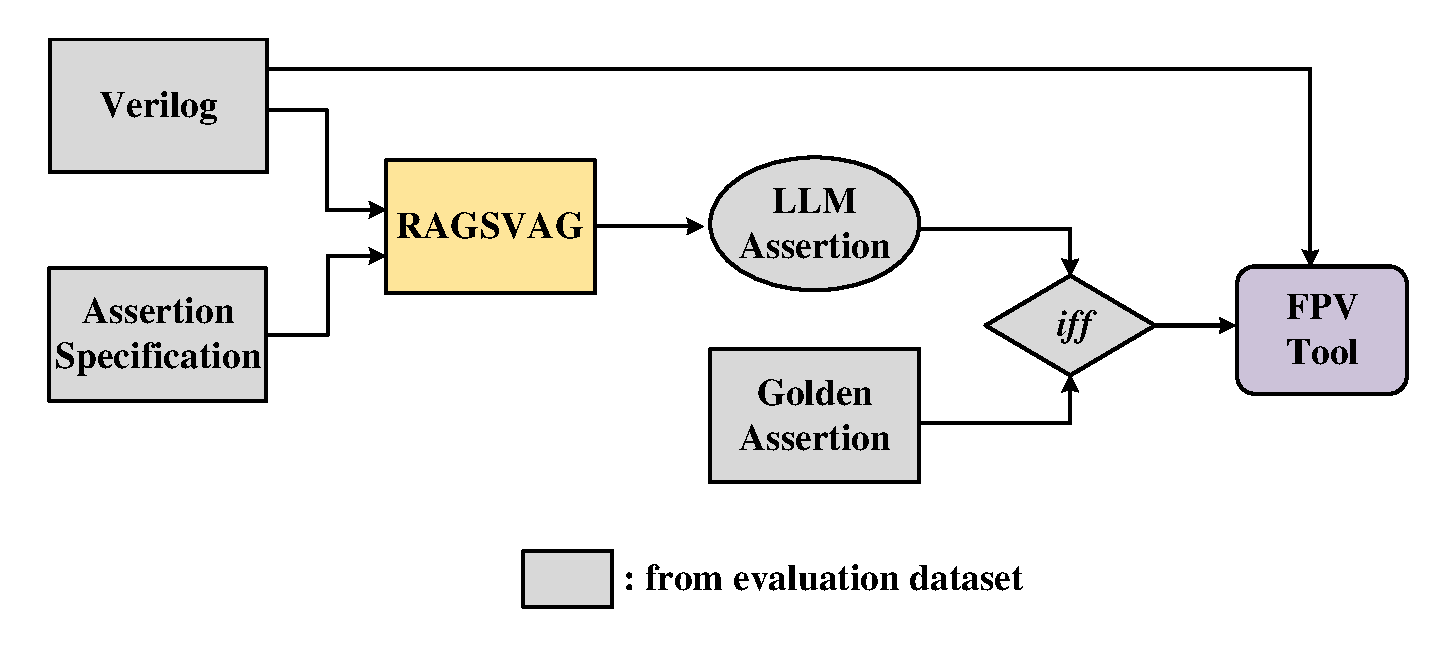
\includegraphics[width=\linewidth]{Figs/Verification_Flow.pdf}
%     \caption{Automatic evaluation framework for LLM-aided SVA generation from natural language.}
%     \label{fig:prompt-assertion-generation-framework}
% \end{figure}

% \subsection{RAG-aided Prompt Assertion Generation}
% \label{subsec:RAG-aided-Assertion-Generation}
% In this section, we aim at using RAG to improve the prompt assertion generation of LLM.

% First, an automatic evaluation framework is proposed for prompt assertion generation, shown in Fig.~\ref{fig:prompt-assertion-generation-framework}.
% The pipeline begins with two key inputs: the Verilog design and its assertion specification, which are both from the evaluation dataset. 
% The two inputs are combined with the output assertion format to construct the \textit{initial prompt}. 
% The template of the initial prompt is shown in Fig.~\ref{fig:Combined-Prompt}.
% Once the LLM assertion is generated, it is compared to a golden assertion from the evaluation dataset, which serves as the reference or ground-truth. 
% To verify that the two assertions are functionally equivalent, they are merged into a single assertion using the SVA syntax \verb|iff|, which is then checked by the FPV tool. 
% If the FPV analysis reveals no counterexamples violating this combined assertion, the LLM assertion is functionally equivalent to the golden one.

% % Once the LLM assertion is produced, it is compared against the golden assertion drawn from the evaluation dataset. 
% % This golden assertion serves as a reference or “ground truth,” ensuring that the assertion generated by the LLM should be functionality-equivalent to the golden one. 
% % The functionality-equivalent checking is realized by:
% % combining the LLM assertion and golden assertion into a new assertion using the SVA syntax \verb|iff|, which is then checked by the FPV tool; 
% % if there is no counterexamples violating the new combined assertion, the LLM assertion is equivalent to the golden one.

% \begin{figure}
%     \centering
%     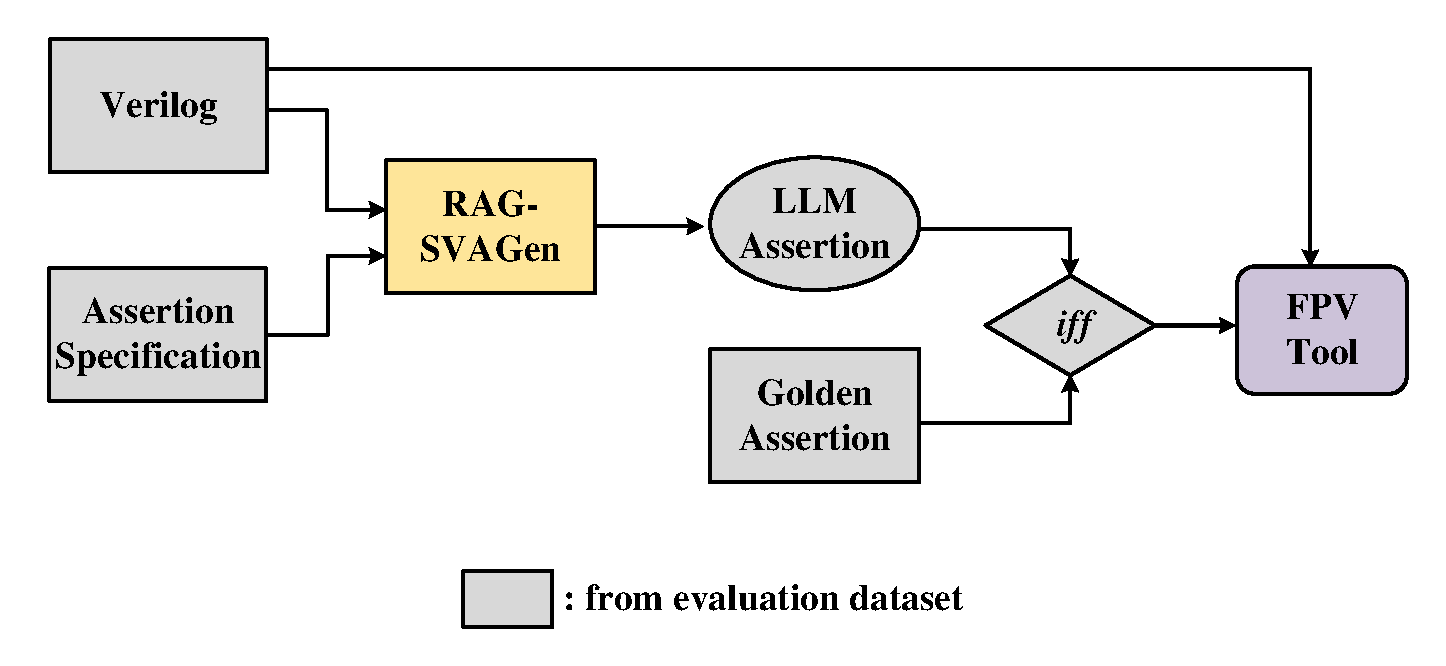
\includegraphics[width=\linewidth]{Figs/Prompt_Assertion_Generation_Flow.pdf}
%     \caption{Automatic evaluation framework for prompt assertion generation.}
%     \label{fig:prompt-assertion-generation-framework}
% \end{figure}

% Next, we will introduce our proposed framework using RAG to provide domain-specific context for prompt assertion generation. 
% As shown in Fig.~\ref{fig:RAG-Prompt-Assertion-Generation}, we construct a RAG database from Verilog textbooks by splitting the contents into chunks. 
% When an assertion specification is given, the RAG framework retrieves the most relevant chunks to augment the user’s initial prompt, ultimately forming a combined prompt that the LLM uses to generate the corresponding SVA. 
% Below, we introduce two proposed splitting techniques for better constructing the database.
% \subsubsection{Static Splitting Technique-based Database}
% In the static splitting approach, the Verilog textbook content is divided into chunks based on a fixed upper bound of characters per chunk. For instance, the text might be segmented every $1000$ characters, ensuring that each chunk remains within a manageable size for embedding and retrieval.
% % Extraction: We first extract the textbook content in its entirety, preserving paragraph boundaries where possible.
% % Chunking: Each block of text is split into pieces once it exceeds the character limit, creating chunks that are large enough to provide context but small enough for efficient retrieval.
% % Embedding and Indexing: Every chunk is converted into a vector embedding using an embedding model (e.g., a transformer-based encoder) and then stored in the RAG database with its metadata (e.g., the page number or section header).
% % Retrieval: At query time, the system calculates the embedding for the user’s prompt and performs a similarity search over all stored embeddings. The top-ranked chunks are retrieved and appended to the user’s initial prompt to form a combined prompt for the LLM.
% Although this method is straightforward and ensures a predictable chunk size, it may inadvertently split related concepts or code snippets, potentially scattering context across multiple chunks.
% \begin{figure}
%     \centering
%     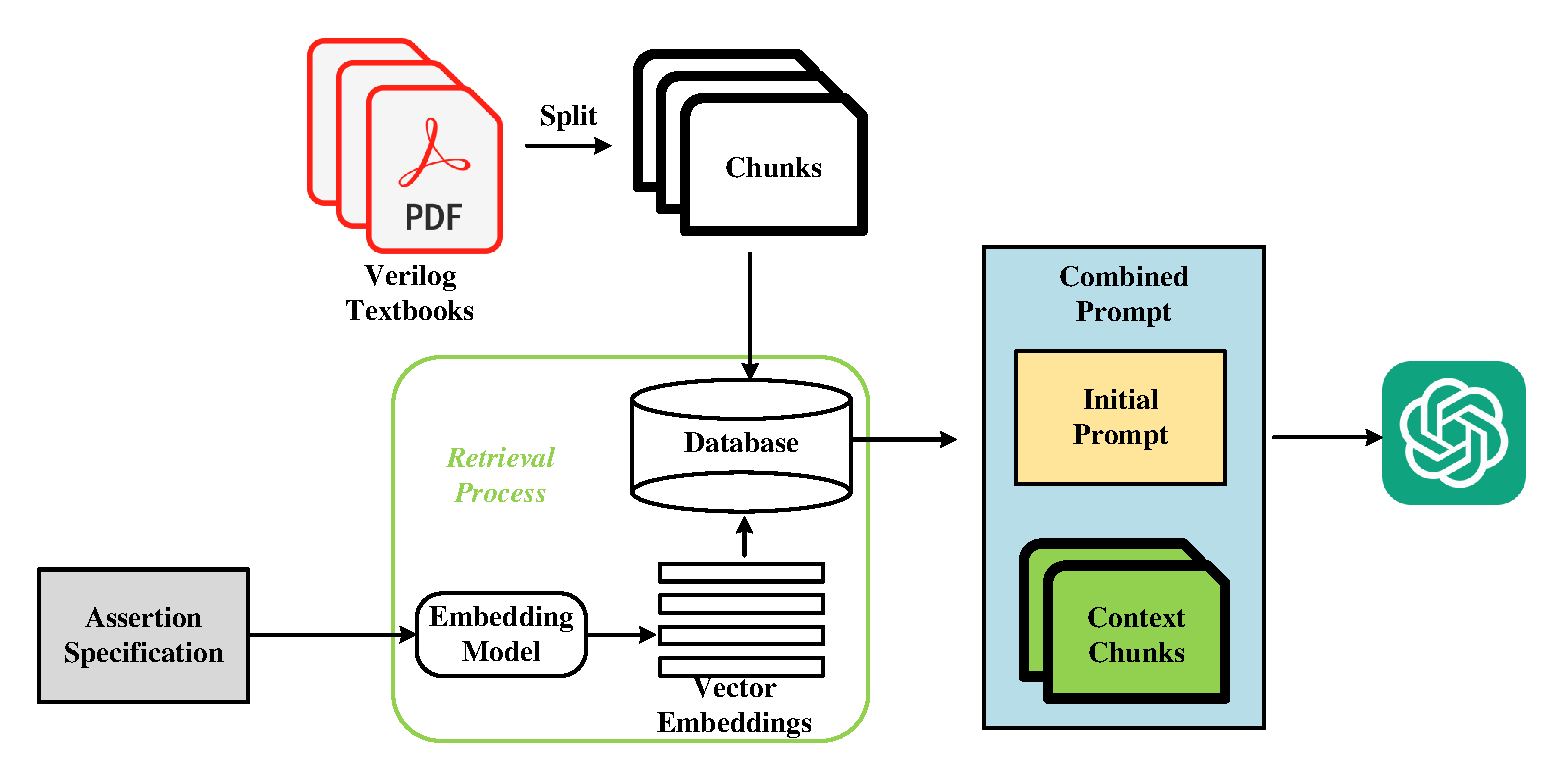
\includegraphics[width=\linewidth]{Figs/RAG_Prompt_Assertion_Generation.pdf}
%     \caption{Framework of RAG-aided prompt assertion generation.}
%     \label{fig:RAG-Prompt-Assertion-Generation}
% \end{figure}
% \subsubsection{Dynamic Splitting Technique-based Database}
% The dynamic splitting technique addresses a key limitation of the static approach by distinguishing between code blocks and explanatory text. 
% It constructs two databases: \textit{Code Database} and \textit{Text Database}.

% Rather than dividing all content at a uniform size threshold, this method begins by parsing the Verilog textbook to locate and isolate code snippets. 
% A font-based detection algorithm, for example, can recognize code segments displayed in a monospace font or other distinctive style. 
% The dynamic splitting technique scans the Verilog textbook for code snippets, using a font-based detection approach to identify lines formatted in a distinct font, such as \textit{Courier}.
% Whenever a code block is detected, it automatically gathers the paragraph immediately preceding the code and the paragraph immediately following it. 
% These three elements—one paragraph before, the code snippet, and one paragraph after—are then combined into a single chunk. By packaging the surrounding paragraphs together with the code, the chunk preserves the immediate context that explains or references the snippet, making it more likely to be useful during retrieval.

% All other text—paragraphs not adjacent to a code block—is split into individual paragraphs and placed in the text database. Each paragraph is processed as its own chunk, enabling the system to retrieve conceptual or theoretical explanations independently. When a user query arrives, the system decides which database to consult based on the query’s nature. If the request involves specific code syntax or an example usage, the code database is queried for the relevant snippet and its neighboring text. Conversely, if the user’s query is more conceptual, the system draws on the text database to provide the appropriate explanatory paragraph(s).

% By splitting content in this manner, the dynamic splitting technique captures local context around code blocks while also making higher-level explanations accessible.


% \begin{figure}
%     \centering
%     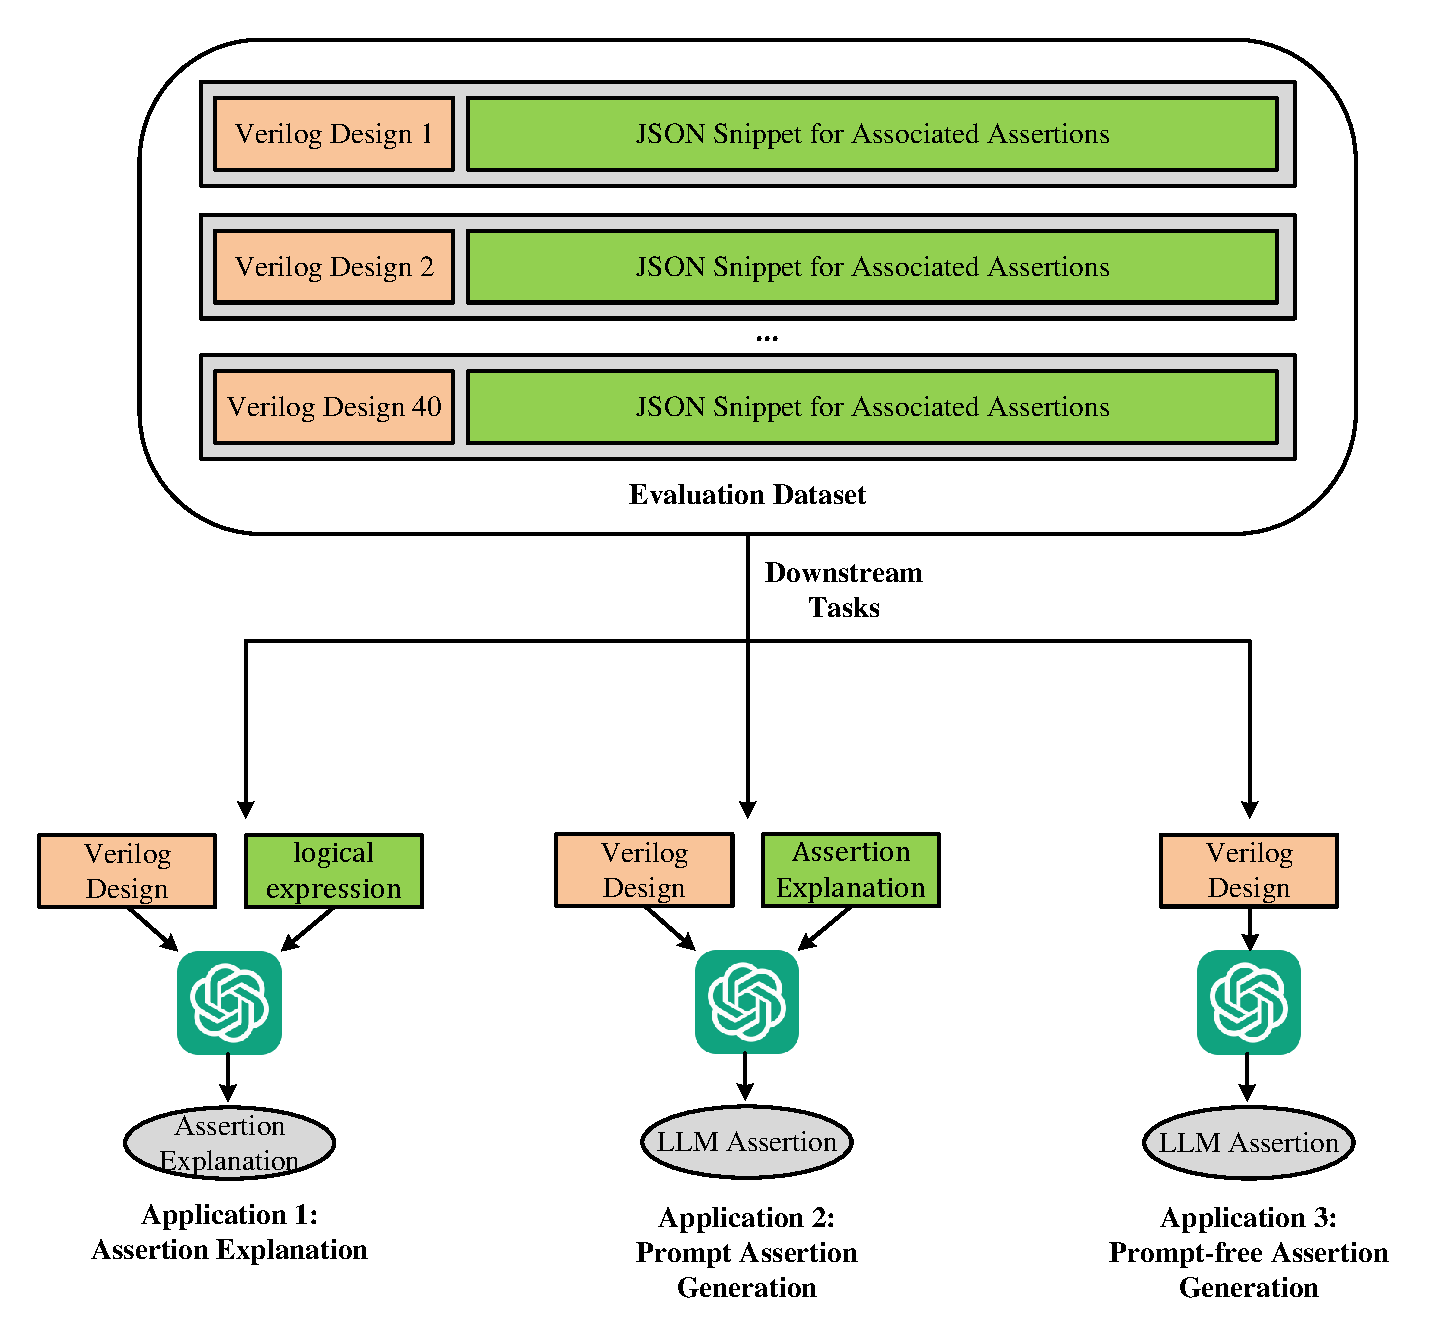
\includegraphics[width=0.8\linewidth]{Figs/Combined_Prompt.pdf}
%     \caption{Combined prompt from RAG framework.}
%     \label{fig:Combined-Prompt}
% \end{figure}


\section{Experimental Results} \label{sec:exp}
\subsection{Experimental Setup}
\label{subsec:experimental-setup}
This experimental section first evaluates the effectiveness of our customized RAG framework for NL2SVA. 
To provide a comprehensive evaluation, we test  it across three LLMs: \textit{OpenAI GPT-4o-mini}, \textit{OpenAI CodeX} which has been fine-tuned on high-quality public code repositories, and \textit{DeepSeek-V3}.
We then evaluate the lightweight \textit{Qwen2.5-Coder-7B-Instruct} model fine-tuned on our synthetic prompt-guided dataset, comparing its performance with the base Qwen model.
We also apply our customized RAG techniques to Qwen and its fine-tuned variants and evaluate their performances.
For methods employing RAG, we retrieve relevant context from the database, which is constructed using $10$ hardware design and verification textbooks.

All experiments are conducted using our evaluation dataset. 
This dataset is the ground truth for evaluating the LLM-generated SVAs in terms of both syntax correctness and functionality match with the natural language property description. 
Two metrics are adopted during evaluation.
\begin{itemize}
    \item \textit{Syntax Correctness (SC)}: number of assertions that are syntactically correct.
    \item \textit{Functionality Match (FM)}: number of assertions that are functionally equivalent to the golden assertions in the evaluation dataset.
\end{itemize}
The two metrics are both derived by the FPV tool \textit{Cadence JasperGold} during our evaluation.
For SC, the FPV tool can directly check the syntax correctness of the LLM-generated SVAs.
For FM, we create the checking SVA by combining the property expression in the golden SVA with that in the LLM-generated SVA using SVA operator \texttt{iff}, as follows:
\begin{verbatim}
     assert property(gold_property_expression 
     iff LLM_property_expression);
\end{verbatim}
If the FPV tool cannot detect any counterexamples for the checking SVA, the two SVAs are functionally equivalent.

Given that our customized RAG framework has multiple components, we perform detailed evaluations on each of them. Specifically, Section~\ref{subsec:exp-evaluation-dynamic} evaluates the effectiveness of the dynamic splitting technique for database construction. 
Section~\ref{subsec:exp-evaluation-hybridretrieval} evaluates the proposed HybridRetrieval method for improving retrieval quality. 
Section~\ref{subsec:exp-evaluate-RAGSVAG} presents an overall evaluation of the customized RAG framework and a comparison with related works.
Finally, Section~\ref{subsec:evaluate-lightweight-llm} evaluates the lightweight Qwen2.5-Coder-7B-Instruct model and its fine-tuned variants using our synthetic dataset, both standalone and integrated with the techniques of our customized RAG framework.

% To assess the effectiveness of the proposed RAG framework, we evaluate both the static splitting technique (\textit{StaticRAG}) and the dynamic splitting technique (\textit{DynamicRAG}) on the prompt-based assertion generation task using our evaluation dataset. 
% To demonstrate the versatility of our framework across different LLMs, we evaluate \textit{OpenAI GPT-4o-mini}, \textit{OpenAI CodeX} which has been fine-tuned on high-quality public code repositories, and \textit{DeepSeek-V3 }, comparing their performance on the assertion generation task. 
% The evaluation is conducted following the automatic framework presented in Fig.~\ref{fig:prompt-assertion-generation-framework}, utilizing Cadence JasperGold~\cite{cadencejaspergold} as the FPV tool to validate both syntax and functionality.
% We use the initial prompt for all methods without using RAG, wile we use the combined prompt for all RAG methods.

% The performance of LLM-generated assertions is measured using the following three metrics:
% \begin{itemize}
%     \item \textit{\#SC} (Syntax Correctness): The number of assertions that are syntactically valid.
%     % \item \#FM (Functionality Correctness): The number of assertions that pass formal verification, meaning no counterexamples exist that violate the assertion.
%     \item \textit{\#FM} (Functionality Match): The number of assertions that are functionally equivalent to the corresponding golden assertions in the dataset.
% \end{itemize}
% Additionally, we evaluate \textit{nl2spec}~\cite{Cosler23}, a related work that employs prompt engineering techniques to improve an LLM’s ability to convert natural language descriptions into temporal logic formulations, which is closely related to SVAs. 
% We modify the prompt of \textit{nl2spec} to be adapted to the SVA generation.
% By including \textit{nl2spec} in our evaluation, we provide a comparative analysis to determine how effective prompt engineering techniques are in enhancing assertion generation accuracy compared to our RAG-aided approach.

\subsection{Evaluation of Dynamic Splitting Technique}
\label{subsec:exp-evaluation-dynamic}
In this subsection, we evaluate the effectiveness of the proposed dynamic splitting technique. 
We compare three methods: applying the base LLM without any retrieval augmentation (\textit{LLM}), applying retrieval augmentation with a database constructed via traditional static splitting (\textit{StaticRAG}), and applying retrieval augmentation with a database constructed using our dynamic splitting  (\textit{DynamicRAG}). 

The evaluation results are summarized in Fig.~\ref{fig:eval-dynamic-splitting}, where the improvement ratio over the basic LLM is shown. 
For GPT-4o-mini, DynamicRAG significantly improves FM by $18.8\%$ compared to LLM, while StaticRAG provides no improvement. 
In terms of SC, DynamicRAG result in $13.5\%$ improvement while StaticRAG only achieves a $2.2\%$ improvement.
When using CodeX, a similar trend is observed. DynamicRAG improves FM by $29.1\%$ over LLM, outperforming StaticRAG ($21.8\%$). 
However, both DynamicRAG and StaticRAG just achieve a slight improvement on SC over LLM.
% SC remains relatively stable across different methods, again suggesting that retrieval augmentation mainly enhances the functional fidelity of generated SVAs.
For DeepSeek, DynamicRAG and StaticRAG even degrade the performance of FM and SC slightly compared to the basic LLM. 
This behavior may be due to DeepSeek’s strong built-in semantic understanding, making it less sensitive to retrieval augmentation quality.
Overall, these results demonstrate that dynamic splitting substantially can help improve the performance of SVA generation for the basic RAG framework.
\begin{figure}
    \centering
    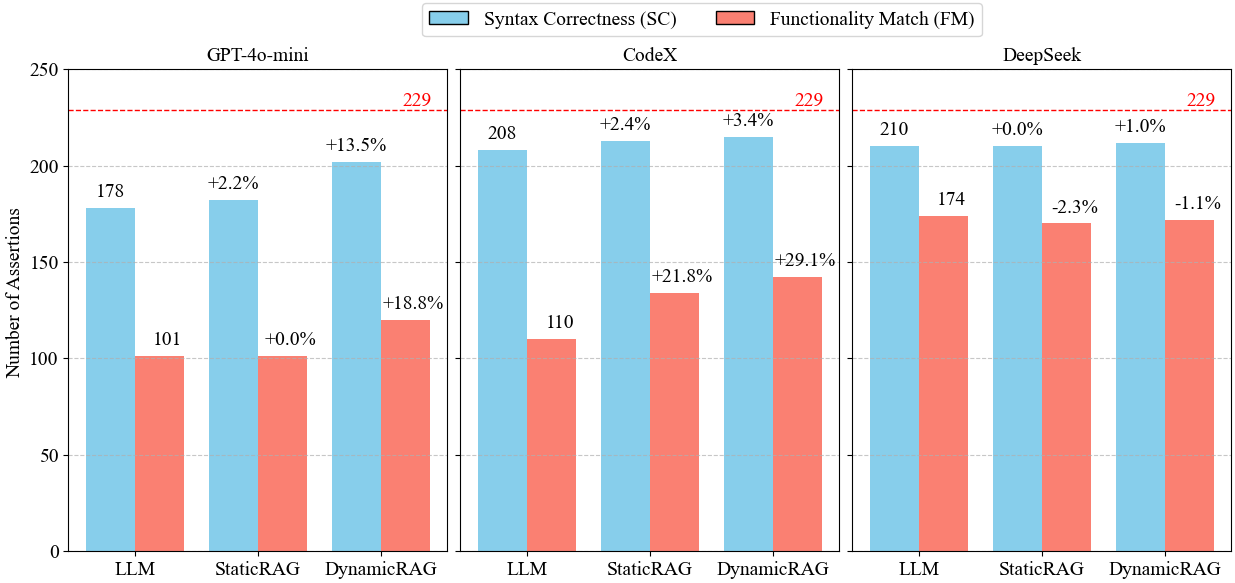
\includegraphics[width=\linewidth]{Figs/exp1_update.png}
    \caption{Evaluation of dynamic splitting technique.}
    \label{fig:eval-dynamic-splitting}
\end{figure}

\subsection{Evaluation of HybridRetrieval}
\label{subsec:exp-evaluation-hybridretrieval}
In this subsection, we evaluate the effectiveness of the proposed HybridRetrieval method. 
Recall that HybridRetrieval consists of the global semantic retrieval and keyword-guided retrieval.
Thus, we compare four methods: (1) using the basic LLM without retrieval augmentation (\textit{LLM}), (2) only global semantic retrieval (\textit{HR-P0}), (3) only keyword-guided retrieval (\textit{HR-P1}), and (4) the full HybridRetrieval (\textit{HR}). In all experiments, the dynamic splitting technique is applied to construct the retrieval database.

The evaluation results are shown in Fig.~\ref{fig:Evaluation-HybridRetrieval}. 
When using GPT-4o-mini, applying HybridRetrieval (both HR-P0 and HR-P1 individually) improves FM substantially compared to the basic LLM. Specifically, HR-P0 improves FM by $18.8\%$ and HR-P1 improves it by $32.7\%$. 
Combining both techniques in HR maintains the $32.7\%$ improvement in FM.
For CodeX, similar trends are observed. HR-P0 and HR-P1 individually improve FM by $18.2\%$ and $19.1\%$, respectively, over the baseline, while the full HybridRetrieval (HR) achieves a $25.5\%$ improvement. 
When evaluating on DeepSeek, improvements are smaller due to the model's stronger built-in understanding ability.  HR still provides consistent FM improvements ($1.1\%$) compared to the baseline, while global semantic retrieval (HR-P0) shows slight $1.1\%$ FM reduction and keyword-guided retrieval (HR-P1) improves by $0.6\%$. 
The full HR yields the best FM performance.

\begin{figure}
    \centering
    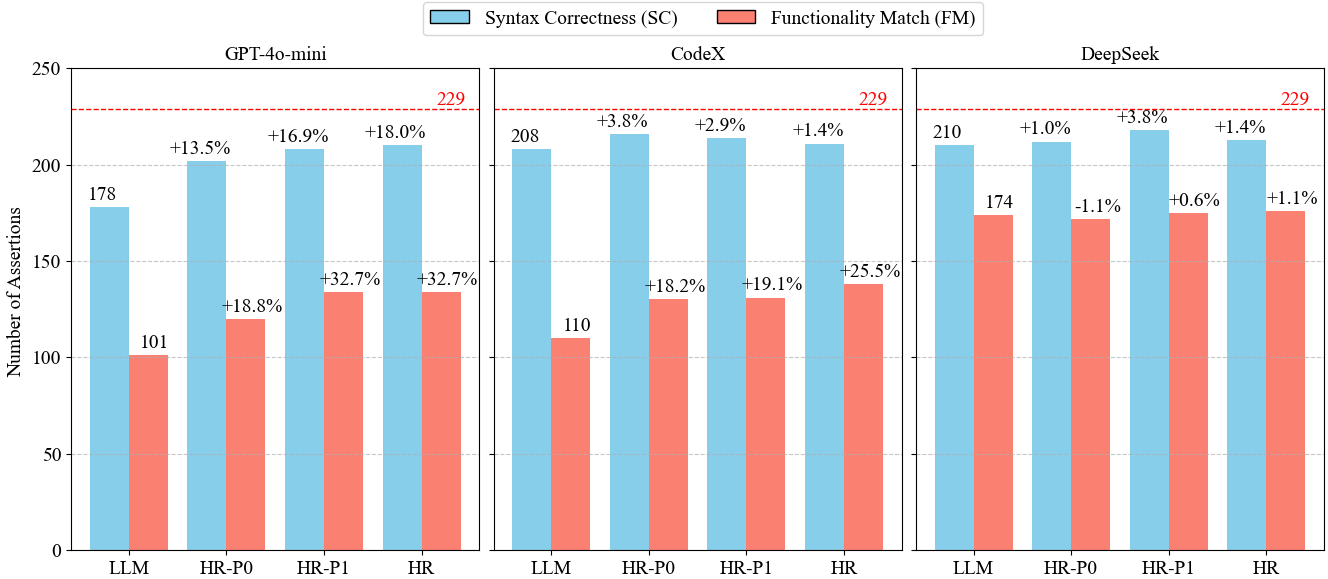
\includegraphics[width=\linewidth]{Figs/exp2_update.png}
    \caption{Evaluation of HybridRetrieval.}
    \label{fig:Evaluation-HybridRetrieval}
\end{figure}

\subsection{Evaluation and Comparison of Customized RAG Framework}
In this subsection, we present the overall evaluation of our full customized RAG framework (\textit{RAGSVAG}) using both HybridRetrieval and SVA operator-based rechecking. Specifically, we do comparison over: applying the plain LLM without any retrieval or augmentation (\textit{LLM}), applying our SVA operator-based rechecking flow without retrieval augmentation (\textit{SOR}), and applying the full RAGSVAG framework. 
For all methods involving RAG, our dynamic splitting technique and HybridRetrieval are employed.
Additionally, we compare our RAGSVAG with \textit{nl2spec}~\cite{Cosler23} and \textit{Spec2Assertion}~\cite{wu2025}.

The results are shown in Fig.~\ref{fig:evaluation-RAGSVAG}. 
Across all the three tested LLMs, RAGSVAG consistently achieves the highest FM among all compared methods, while maintaining competitive SC.
For GPT-4o-mini, applying nl2spec improves FM by $8.9\%$ and applying Spec2Assertion improves FM by $6.9\%$, while SOR alone improves it by $30.7\%$. In contrast, RAGSVAG achieves a FM improvement of $58.4\%$, representing a substantial gain over both baseline and intermediate methods.
For CodeX, similar trends are observed. 
Applying nl2spec improves FM by $18.2\%$ and applying Spec2Assertion improves FM by $25.5\%$, and SOR improves it by $20.0\%$. RAGSVAG can achieve a $34.5\%$ improvement over FM,  outperforming the baselines.
For DeepSeek, which shows strong baseline performance, relative improvements are smaller.  RAGSVAG still achieves a FM improvement of $10.9\%$ compared to the basic LLM, while SOR provide smaller gains, and the nl2spec and Spec2Assertion actually underperform relative to the baseline.
In terms of SC, all methods show smaller improvement, indicating that retrieval and rechecking enhance the FC accuracy of the generated assertions rather than SC.
Overall, the results demonstrate the effectiveness of RAGSVAG in substantially improving the FM of LLM-generated SVAs.

\label{subsec:exp-evaluate-RAGSVAG}
\begin{figure}
    \centering
    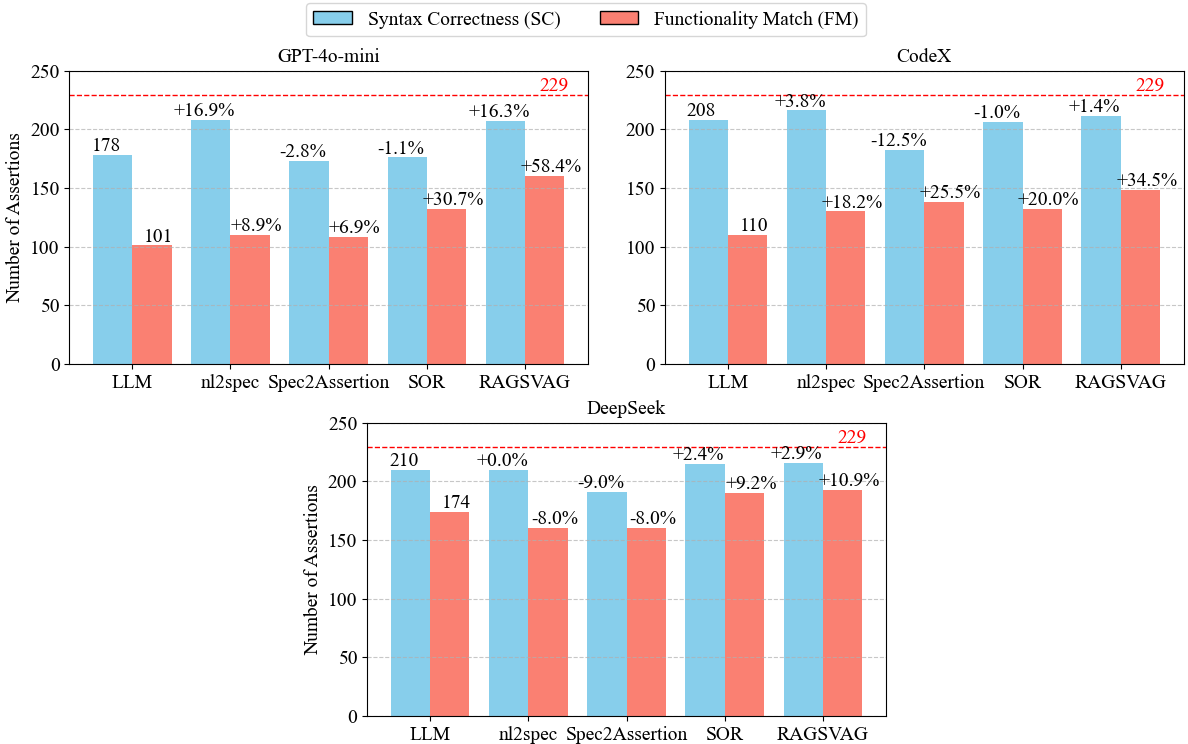
\includegraphics[width=\linewidth]{Figs/exp3_update_1.png}
    \caption{Evaluation and comparison of Customized RAG Framework.}
    \label{fig:evaluation-RAGSVAG}
\end{figure}

\subsection{Evaluation of Finetuned Lightweight LLM}
\label{subsec:evaluate-lightweight-llm}
We evaluate the lightweight \textit{Qwen2.5-Coder-7B-Instruct} model~\cite{hui24} and two fine-tuned variants derived from our synthetic finetuning Dataset in Section~\ref{subsec:synthetic-finetuning-dataset}.  
The first variant, \textit{Qwen-Finetune}, is trained on plain (\emph{SVA, explanation}) pairs from our finetuning dataset following~\cite{Shahidzadeh24}.  
The second, \textit{Qwen-Prompt-Finetune}, is trained on (\emph{SVA, prompt-guided explanation}) pairs.  
The two fine-tuning tasks use supervised learning with \textit{Llama-Factory} \cite{zheng2024llamafactory}, a cosine learning-rate schedule, an initial rate of $8\times10^{-5}$, \texttt{bf16} precision and three epochs.  
Training the two variants on $8 \times$ A100 GPUs requires roughly two hours.

We integrate the techniques from our customised RAG framework into the base Qwen model and its two fine-tuned variants. 
We employ Qwen and its fine-tuned variants with a temperature of $0.6$, top\_p of $0.95$. Considering the format of our fine-tuning dataset and Qwen’s limited context window, we  feed the assertion specification together with the related signals and their natural language explanations, rather than the full Verilog code, into the model or RAG pipeline.

Table \ref{tab:qwen_results} reports results of SC and FM, the corresponding percentages relative to all $229$ SVAs, and the improvements achieved with respect to the base model.
The first column reports the results of the base Qwen. 
The model produces $161$ SC and $105$ FM SVAs, or $70.31 \%$ and $45.85 \%$ of the $229$ SVAs. 
Integrating HybridRetrieval  improves the two metrics to $198$ / $113$. 
Integrating our SVA operator-based rechecking achieves higher SC to $201$ but decreases FM to $101$, and integrating our customized RAG framework ends at $195$ / $101$. 
In short, the base model achieves similar SVA generation performance to that of GPT-4o-mini and benefits from HybridRetrieval, while the SVA operator-based rechecking components help improve SC.

The second column reports the results of Qwen-Finetune. This variant falls to $160$ / $87$, losing $0.62 \%$ in SC and $17.14 \%$ in FM compared with the base model, so we do not integrated any techniques into it. 
By contrast, the third column Qwen-Prompt-Finetune improves SC / FM to $206$ / $148$ ($89.96 \%$ / $64.63 \%$), a $27.95 \%$ SC gain and a $40.95 \%$ FM gain over the base model. 
When HybridRetrieval is integrated, the two metrics continue to be improved to $213$ / $167$, and they remain well above the baseline integrating SVA operator-based rechecking and the overall customized RAG framework. 
These results confirm that fine-tuning the lightweight Qwen model with prompt-guided explanations markedly improves SVA generation, and that integrating the HybridRetrieval component of our customized RAG framework provides an additional improvement.
\begin{table}[t]
\centering
\caption{Evaluation results of the base Qwen model, its finetuned variant, and its prompt-finetuned variant, each used together with our customised RAG framework.}
\label{tab:qwen_results}
% \newcommand{\tabincell}[2]{\begin{tabular}[c]{@{}#1@{}}#2\end{tabular}}
\setlength{\tabcolsep}{1.5pt}
\renewcommand{\arraystretch}{1.35}
\begin{tabular}{@{}lcc cc cc@{}}
\toprule
\multirow{2}{*}{Methods} &
\multicolumn{2}{c}{Qwen} &
\multicolumn{2}{c}{Finetune-Qwen} &
\multicolumn{2}{c}{Prompt-Finetune-Qwen} \\ \cmidrule(lr){2-3}\cmidrule(lr){4-5}\cmidrule(l){6-7}
 & SC & FM & SC & FM & SC & FM \\ \midrule
LLM     & \tabincell{c}{161\\(70.31\%)} & \tabincell{c}{105\\(45.85\%)} & \tabincell{c}{160\\(69.87\%)} & \tabincell{c}{87\\(37.99\%)}  & \tabincell{c}{206\\(89.96\%)} & \tabincell{c}{148\\(64.63\%)} \\
\textit{Improv.} & --- & --- & -0.62\% & -17.14\% & +27.95\% & +40.95\% \\[1ex]
\hline
HR      & \tabincell{c}{198\\(86.46\%)} & \tabincell{c}{113\\(49.34\%)} & --- & --- & \tabincell{c}{\textbf{213}\\(\textbf{93.01\%})} & \tabincell{c}{\textbf{167}\\(\textbf{72.93\%})} \\
\textit{Improv.} & +22.98\% & +7.62\% & --- & --- & \textbf{+32.30}\% & \textbf{+59.05}\% \\[1ex]
\hline
SOR     & \tabincell{c}{201\\(87.77\%)} & \tabincell{c}{101\\(44.10\%)} & --- & --- & \tabincell{c}{208\\(90.83\%)} & \tabincell{c}{155\\(67.69\%)} \\
\textit{Improv.} & +24.84\% & -3.81\% & --- & --- & +29.19\% & +47.62\% \\[1ex]
\hline
RAGSVAG & \tabincell{c}{195\\(85.15\%)} & \tabincell{c}{101\\(44.10\%)} & --- & --- & \tabincell{c}{211\\(92.14\%)} & \tabincell{c}{164\\(71.62\%)} \\
\textit{Improv.} & +21.12\% & -3.81\% & --- & --- & +31.06\% & +56.19\% \\ \bottomrule
\end{tabular}
\end{table}


% Fig.~\ref{fig:GPT-4o-mini} and~\ref{fig:GPT-4o} present comparative experimental results of different methods using \textit{GPT-4o-mini} and \textit{CodeX}, respectively. 
% We evaluate these methods based on the three critical metrics \#SC, \#FM, and \#FM.

% As depicted in Fig.~\ref{fig:GPT-4o-mini}, using \textit{GPT-4o-mini} as the baseline, we observe that the \textit{nl2spec} method significantly enhances performance, achieving a $16.9\%$ improvement in \#SC, along with notable gains in \#FM ($7.8\%$) and \#FM ($8.9\%$). 
% The \textit{StaticRAG} method, however, yields only marginal improvement ($2.2\%$) in \#SC, with no observable change in \#FM and \#FM. 
% In contrast, the \textit{DynamicRAG} method demonstrates substantial performance enhancements across all metrics, achieving improvements of $13.5\%$ in \#SC, $18.6\%$ in \#FM, and $18.8\%$ in \#FM, clearly highlighting its effectiveness over \textit{StaticRAG}.

% In Fig.~\ref{fig:GPT-4o}, it shows similar experiments conducted with \textit{CodeX} as the baseline model. 
% Here, the \textit{nl2spec} method moderately increases \#SC by $3.8\%$, and significantly boosts \#FM and \#FM by $18.0\%$ and $18.2\%$, respectively. 
% \textit{StaticRAG} achieves comparable but slightly lower gains in \#SC ($2.4\%$), but substantially higher improvements in \#FM and \#FM ($21.6\%$ and $21.8\%$, respectively). 
% The \textit{DynamicRAG} method surpasses all other approaches, delivering the highest improvements observed: $3.4\%$ in \#SC, $28.8\%$ in \#FM, and $29.1\%$ in \#FM. 
% These results underscore \textit{DynamicRAG}'s consistent advantage, showing its ability to notably enhance the capabilities of \textit{CodeX}.

% Overall, the experimental analysis clearly indicates that augmenting the two baseline LLMs with the \textit{DynamicRAG} method consistently delivers better performance across all measured criteria, proving its practical effectiveness for improving LLM-aided assertion generation.


% \begin{figure}
%     \centering
%     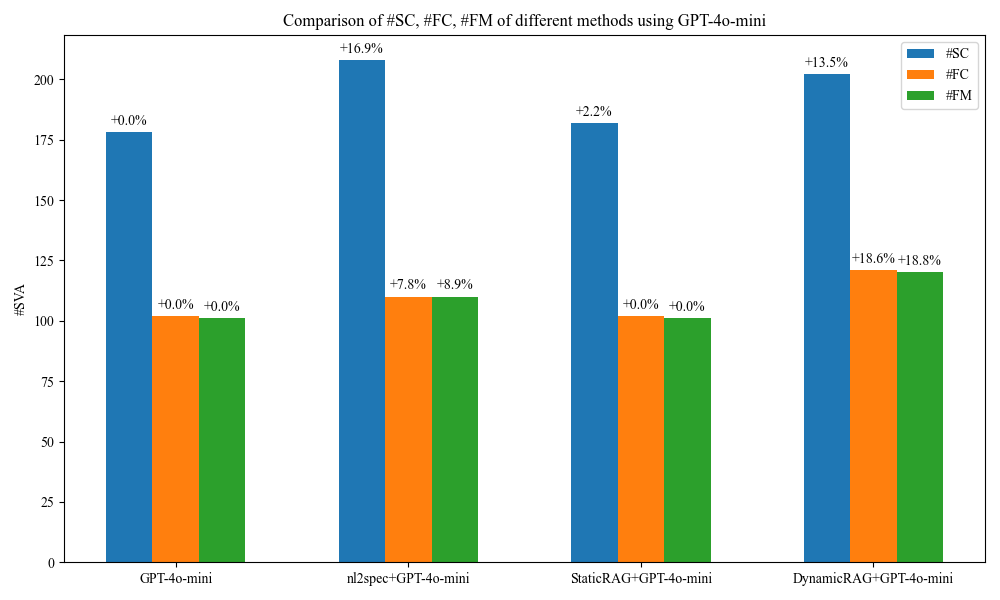
\includegraphics[width=\linewidth]{Figs/Figure_1.png}
%     \caption{Comparison of \#SC, \#FM, \#FM of different methods using \textit{GPT-4o-mini}.}
%     \label{fig:GPT-4o-mini}
% \end{figure}

% \begin{figure}
%     \centering
%     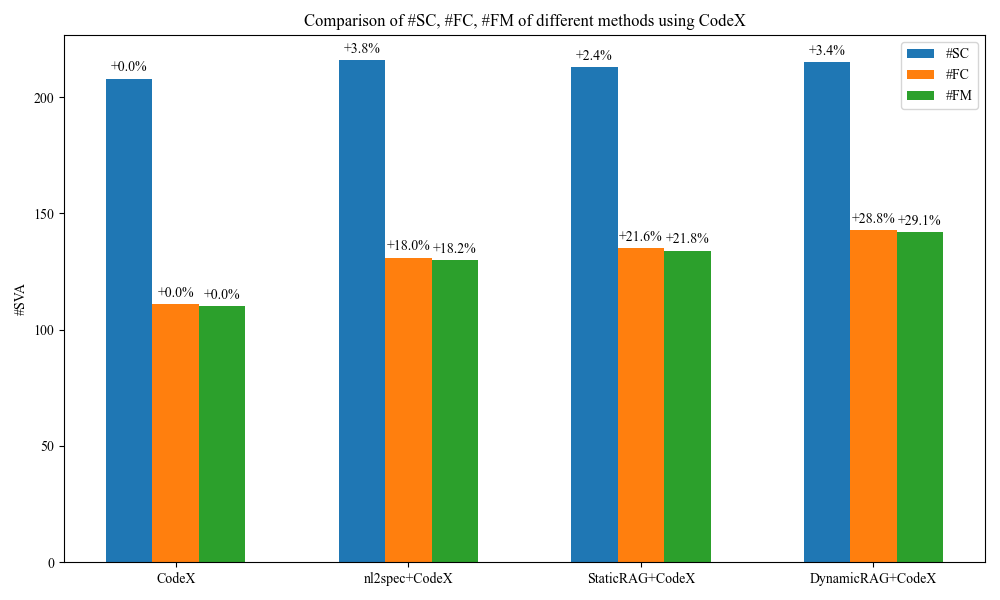
\includegraphics[width=\linewidth]{Figs/Figure_2.png}
%     \caption{Comparison of \#SC, \#FM, \#FM of different methods using \textit{CodeX}.}
%     \label{fig:GPT-4o}
% \end{figure}

% \subsection{Example SVAs Generated by RAGSVAG}
% \label{subsec:exp-example-svas}
% To  illustrate the effectiveness of RAGSVAG, we select $10$ natural language property explanations from our evaluation dataset. 
% For each explanation, we show the corresponding SVAs generated by the baseline GPT-4o-mini and by RAGSVAG, as summarized in Table~\ref{tab:example_svas}. 
% In addition, we provide the  design name and the number of lines in the Verilog code for each example, offering more context about the complexity of the design where the property originates.

% Each generated assertion is further validated using the proposed assertion verification framework described in Section~\ref{subsec:Evaluation-Dataset}. Specifically, we check whether the generated SVA correctly matches the intended functionality described in the natural language property.
% Across all $10$ examples, the SVAs generated by RAGSVAG pass the functionality verification, meaning they accurately implement the property. In contrast, the SVAs generated by GPT-4o-mini exhibit functionality mismatches in every case.  Common issues include incorrect usage of temporal operators (such as overlapping implication operator \texttt{|->} and non-overlapping implications operator \texttt{|=>}), improper handling of past signal values, and failure to accurately capture the specified clock-cycle timing relationships.

% % \begin{table*}[ht]
% %     \centering
% %     \caption{Examples of SVAs generated by GPT-4o-mini and RAGSVAG.}
% %     \label{tab:example_svas}
% %     \begin{tabular}{|c|c|p{3.8cm}|p{5.4cm}|p{5.4cm}|}
% %         \hline
% %         \textbf{Design} & \textbf{Lines} & \textbf{Natural Language Property} & \textbf{GPT-4o-mini SVA} & \textbf{RAGSVAGen SVA} \\
% %         \hline
% %         ff & $10$ & When enable signal is set (1), output equals input from previous cycle in next cycle. & \texttt{assert property (@(posedge clk) disable iff (rst) (en == 1'b1 |=> out == in[1]));} & \texttt{assert property (@(posedge clk) disable iff (rst) (en |=> (out == \$past(in))));} \\
% %         \hline
% %         pwm & $18$ & Eventually, the inversion of the output becomes true. & \texttt{assert property (@(posedge clk) (s\_eventually (!pulse)));} & \texttt{assert property (@(posedge clk) (pulse |-> eventually (!pulse)));} \\
% %         \hline
% %         register & $20$ & When enable reset (0), output equals last output in next cycle. & \texttt{assert property (@(posedge clk) disable iff (rst) (en == 0 |-> out == out[1]));} & \texttt{assert property (@(posedge clk) disable iff (rst) (en == 0 |=> (out == \$past(out))));} \\
% %         \hline
% %         simple\_req\_ack & $31$ & When request signal is detected to have a rising edge, then after a delay of $2$ clock cycles the acknowledge signal is detected to have a rising edge. & \texttt{assert property (@(posedge clk) disable iff(!rst\_n) (req\_ff in \{1'b0, 1'b1\} during [2] |=> (ack\_ff == 1'b1)));} & \texttt{assert property (@(posedge clk) disable iff(!rst\_n) (\$rose(req) |=> \#\#2 \$rose(ack)));} \\
% %         \hline
% %         or1200\_if & $194$ & When pipeline flush signal is reset ($0$) and save instruction condition is true, then saved flag equals 1 in the next clock cycle. & \texttt{assert property (@(posedge clk) disable iff (rst) (if\_flushpipe == 0 \&\& save\_insn |-> saved));} & \texttt{assert property (@(posedge clk) disable iff (rst) (if\_flushpipe == 0 \&\& save\_insn |=> (saved == 1)));} \\
% %         \hline
% %         arbiter & $231$ & When the first bit of grant output is asserted and in the previous clock cycle the arbitration type selector signal was equal to $0$, then the first bit of request input signal from the previous clock cycle must be asserted in the current clock cycle. & \texttt{assert property (@(posedge clk) disable iff (\textasciitilde rst\_n) (gnt[0] \&\& arb\_type == 0 |-> req[0]));} & \texttt{assert property (@(posedge clk) disable iff (\textasciitilde rst\_n) ((gnt[0] \&\& \$past(arb\_type) == 0) |-> \$past(req[0])));} \\
% %         \hline
% %         a25\_wishbone & $447$ & When the wishbone bus state equals \texttt{WB\_BURST1} and the acknowledgement signal is asserted, then the wishbone bus state equals \texttt{WB\_BURST2} in the next clock cycle. & \texttt{assert property (@(posedge i\_clk) (wishbone\_st == WB\_BURST1 \&\& i\_wb\_ack |-> (wishbone\_st == WB\_BURST2)));} & \texttt{assert property (@(posedge i\_clk) ((wishbone\_st == WB\_BURST1 \&\& i\_wb\_ack) |=> (wishbone\_st == WB\_BURST2)));} \\
% %         \hline
% %         control\_unit & $602$ & When the signal that indicates the beginning of an AES operation equals 0, then the signal used to initialize the key generation process equals 0 in the current clock cycle. & \texttt{assert property (@(posedge clk) (start == 0 |=> key\_init == 0));} & \texttt{assert property (@(posedge clk) (start == 1'b0 |-> key\_init == 1'b0));} \\
% %         \hline
% %         or1200\_ctrl & $1225$ & When the freeze signal for the EX stage is reset ($0$) and either the freeze signal for the ID stage is set ($1$) or the pipeline flush signal for the EX stage is set ($1$), then the signal indicating a MAC read operation in the EX stage equals 0 in the next clock cycle. & \texttt{assert property (@(posedge clk) disable iff (rst) (!ex\_freeze \&\& (id\_freeze || ex\_flushpipe) |-> (ex\_macrc\_op == 0)));} & \texttt{assert property (@(posedge clk) disable iff (rst) ((!ex\_freeze \&\& (id\_freeze || ex\_flushpipe)) |=> (ex\_mac\_op == 0)));} \\
% %         \hline
% %         module\_i2c & $3382$ & When the FIFO receiver empty indicator equals $1$, then the FIFO receiver empty output equals $1$ in the current clock cycle. & \texttt{assert property (@(posedge PCLK) (fifo\_rx\_f\_empty == 1'b1 |-> fifo\_rx\_wr\_en == 1'b1));} & \texttt{assert property (@(posedge PCLK) (fifo\_rx\_f\_empty == 1'b1 |-> RX\_EMPTY == 1'b1));} \\
% %         \hline
% %     \end{tabular}
% % \end{table*}

% % \subsection{Evaluation Results over CodeLlama}
% % \label{subsec:results-over-CodeLlama}
% % In Fig.~\ref{fig:CodeLlama}, it illustrates the performance of augmentation methods with \textit{CodeLlama} as the baseline. 
% % \textit{CodeLlama} initially demonstrates considerably poorer performance compared to \textit{OpenAI} models across all metrics. 
% % To mitigate this, prompts are augmented with used signals for each golden assertion, represented by lighter-colored portions of each bar, which reflect the quantitative improvements after adding signals into the prompt. 
% % Note that the used signals can be directly extracted from our evaluation dataset.
% % Notably, the \textit{StaticRAG} method with signals slightly improves \#SC by $0.5\%$, while achieving meaningful gains in \#FM ($5.0\%$) and \#FM ($5.1\%$). 
% % The \textit{DynamicRAG} method yields a small decrease in \#SC ($-1.5\%$) but provides substantial improvements in \#FM ($8.0\%$) and \#FM ($8.1\%$), indicating the effectiveness of including used signals in enhancing assertion generation. 
% % Thus, identifying relevant signals from Verilog code is crucial for assertion generation and relies heavily on the code explanation capability of an LLM. 
% % \textit{CodeLlama}, however, exhibits limitations in this regard.


\section{Conclusion} \label{sec:con}
In this paper, we present a customized RAG framework and a synthetic fine-tuning dataset of prompt-guided explanations to streamline SVA generation from natural language descriptions. The RAG framework integrates dynamic splitting, HybridRetrieval, and an operator-based rechecking flow for precise context retrieval and assertion validation, while the dataset provides layer-by-layer explanation of each SVA spanning the Boolean, sequence, property, and verification layers. 
We also construct the largest evaluation dataset for NL2SVA to date, with $40$ Verilog designs and $229$ formally verified assertions with detailed annotations.
Evaluation on GPT-4o-mini, CodeX, DeepSeek-V3, and a fine-tuned Qwen2.5-Coder-7B-Instruct model shows that combining our customized RAG framework with prompt-guided fine-tuning delivers marked improvements in syntax correctness and functionality match, enabling robust SVA synthesis with minimal manual effort.

% This paper presents RAG-SVAGen, a retrieval-augmented generation framework designed to improve the quality of SVA generation from natural language property descriptions. To address the challenges of domain-specific syntax and semantics in hardware verification, RAGSVAG integrates three proposed key techniques: a dynamic splitting method, a HybridRetrieval mechanism that combines global semantic retrieval with keyword-guided retrieval, and an SVA operator-based rechecking flow.
% To rigorously evaluate the RAGSVAG framework, we construct the largest evaluation dataset for natural language to SVA translation to date, with 40 Verilog designs and 229 formally verified assertions with detailed annotations. We  develop an automatic evaluation framework that validates syntax correctness and functionality match using FPV tools.
% Experimental results across multiple LLMs show that RAGSVAG substantially improves functionality match baseline LLMs and a related work, advancing the automation of assertion-based hardware verification.
% \newpage
%This paper presents RAGSVAG, a retrieval-augmented generation framework that enhances LLM-based SystemVerilog assertion generation from natural language descriptions. RAGSVAG integrates a dynamic splitting technique for database construction, a HybridRetrieval mechanism combining semantic and keyword-guided retrieval, and an SVA operator-based rechecking flow to refine generated assertions. To support systematic evaluation, we construct the largest known dataset for natural language to SVA translation and develop an automatic verification framework. Experimental results across multiple LLMs show that RAGSVAG substantially improves functionality match baseline LLMs and a related work, advancing the automation of assertion-based hardware verification.



% This paper advances the automation of SVA generation by introducing a comprehensive evaluation dataset, an automatic evaluation framework, and a RAG framework for improving LLM assertion generation. 
% Our evaluation dataset, the largest of its kind to our knowledge, comprises $40$ Verilog designs and $229$ verified assertions, each with detailed annotations, enabling evaluation of LLM-based assertion generation at different levels. 
% The proposed evaluation framework automatically checks the functionality equivalence between the LLM-generated assertions and the reference assertions from our evaluation dataset using the FPV tool. 
% To enhance assertion generation ability of LLM, we construct a RAG database from Verilog textbooks and introduce two text-splitting techniques—static and dynamic—to improve contextual retrieval. The dynamic approach, which separates code and text databases, preserves assertion-related knowledge more effectively, leading to improved LLM performance.
% Despite these advancements, challenges remain in fully automating assertion generation for highly complex or evolving design specifications. Future work can explore improved retrieval mechanisms, adaptive prompting strategies, and deeper integration of formal verification feedback into the generation process. Nonetheless, our contributions—a large-scale, richly annotated dataset, an objective evaluation pipeline, and a RAG-based retrieval framework—provide a strong foundation for advancing LLM-driven assertion generation and its applications in hardware verification.
% \input{Tex/Acknowledgment}
\bibliographystyle{IEEEtran}
\bibliography{Reference}
\onecolumn
\newpage
\appendix

% \section{Appendix}
\subsection{Example SVAs}
\label{subsec:Example-SVAs}
Across all $10$ examples in Table~\ref{tab:example_svas}, the SVAs generated by our customized RAG framework pass the functionality verification, meaning they accurately implement the property. In contrast, the SVAs generated by GPT-4o-mini exhibit functionality mismatches in every case.  Common issues include incorrect usage of temporal operators (such as overlapping implication operator \texttt{|->} and non-overlapping implications operator \texttt{|=>}), improper handling of past signal values, and failure to accurately capture the specified clock-cycle timing relationships.
\begin{table*}[ht]
    \centering
    \caption{Examples of SVAs generated by GPT-4o-mini and RAGSVAG.}
    \label{tab:example_svas}
    \begin{tabular}{|c|c|p{3.8cm}|p{5.4cm}|p{5.4cm}|}
        \hline
        \textbf{Design} & \textbf{Lines} & \textbf{Natural Language Explanation} & \textbf{GPT-4o-mini SVA} & \textbf{RAGSVAG SVA} \\
        \hline
        ff & $10$ & When enable signal is set (1), output equals input from previous cycle in next cycle. & \texttt{assert property (@(posedge clk) disable iff (rst) (en == 1'b1 |=> out == in[1]));} & \texttt{assert property (@(posedge clk) disable iff (rst) (en |=> (out == \$past(in))));} \\
        \hline
        PWM & $18$ & Eventually, the inversion of the output becomes true. & \texttt{assert property (@(posedge clk) (pulse |-> eventually (!pulse)));} & \texttt{assert property (@(posedge clk) (s\_eventually (!pulse)));}\\
        \hline
        register & $20$ & When enable reset (0), output equals last output in next cycle. & \texttt{assert property (@(posedge clk) disable iff (rst) (en == 0 |-> out == out[1]));} & \texttt{assert property (@(posedge clk) disable iff (rst) (en == 0 |=> (out == \$past(out))));} \\
        \hline
        simple\_req\_ack & $31$ & When request signal is detected to have a rising edge, then after a delay of $2$ clock cycles the acknowledge signal is detected to have a rising edge. & \texttt{assert property (@(posedge clk) disable iff(!rst\_n) (req\_ff in \{1'b0, 1'b1\} during [2] |=> (ack\_ff == 1'b1)));} & \texttt{assert property (@(posedge clk) disable iff(!rst\_n) (\$rose(req) |=> \#\#2 \$rose(ack)));} \\
        \hline
        or1200\_if & $194$ & When pipeline flush signal is reset ($0$) and save instruction condition is true, then saved flag equals 1 in the next clock cycle. & \texttt{assert property (@(posedge clk) disable iff (rst) (if\_flushpipe == 0 \&\& save\_insn |-> saved));} & \texttt{assert property (@(posedge clk) disable iff (rst) (if\_flushpipe == 0 \&\& save\_insn |=> (saved == 1)));} \\
        \hline
        arbiter & $231$ & When the first bit of grant output is asserted and in the previous clock cycle the arbitration type selector signal was equal to $0$, then the first bit of request input signal from the previous clock cycle must be asserted in the current clock cycle. & \texttt{assert property (@(posedge clk) disable iff (\textasciitilde rst\_n) (gnt[0] \&\& arb\_type == 0 |-> req[0]));} & \texttt{assert property (@(posedge clk) disable iff (\textasciitilde rst\_n) ((gnt[0] \&\& \$past(arb\_type) == 0) |-> \$past(req[0])));} \\
        \hline
        a25\_wishbone & $447$ & When the wishbone bus state equals \texttt{WB\_BURST1} and the acknowledgement signal is asserted, then the wishbone bus state equals \texttt{WB\_BURST2} in the next clock cycle. & \texttt{assert property (@(posedge i\_clk) (wishbone\_st == WB\_BURST1 \&\& i\_wb\_ack |-> (wishbone\_st == WB\_BURST2)));} & \texttt{assert property (@(posedge i\_clk) ((wishbone\_st == WB\_BURST1 \&\& i\_wb\_ack) |=> (wishbone\_st == WB\_BURST2)));} \\
        \hline
        control\_unit & $602$ & When the signal that indicates the beginning of an AES operation equals 0, then the signal used to initialize the key generation process equals 0 in the current clock cycle. & \texttt{assert property (@(posedge clk) (start == 0 |=> key\_init == 0));} & \texttt{assert property (@(posedge clk) (start == 1'b0 |-> key\_init == 1'b0));} \\
        \hline
        or1200\_ctrl & $1225$ & When the freeze signal for the EX stage is reset ($0$) and either the freeze signal for the ID stage is set ($1$) or the pipeline flush signal for the EX stage is set ($1$), then the signal indicating a MAC read operation in the EX stage equals 0 in the next clock cycle. & \texttt{assert property (@(posedge clk) disable iff (rst) (!ex\_freeze \&\& (id\_freeze || ex\_flushpipe) |-> (ex\_macrc\_op == 0)));} & \texttt{assert property (@(posedge clk) disable iff (rst) ((!ex\_freeze \&\& (id\_freeze || ex\_flushpipe)) |=> (ex\_mac\_op == 0)));} \\
        \hline
        module\_i2c & $3382$ & When the FIFO receiver empty indicator equals $1$, then the FIFO receiver empty output equals $1$ in the current clock cycle. & \texttt{assert property (@(posedge PCLK) (fifo\_rx\_f\_empty == 1'b1 |-> fifo\_rx\_wr\_en == 1'b1));} & \texttt{assert property (@(posedge PCLK) (fifo\_rx\_f\_empty == 1'b1 |-> RX\_EMPTY == 1'b1));} \\
        \hline
    \end{tabular}
\end{table*}


\subsection{Prompt-guided Explanation Generation}
\label{subsec:prompt-guided-explanation-generation}
The prompt for generating the prompt-guided explanation of the given golden SVA and natural language explanation is shown in Fig.~\ref{fig:prompt-guided-explanation-generation}. 
\begin{figure}
    \centering
    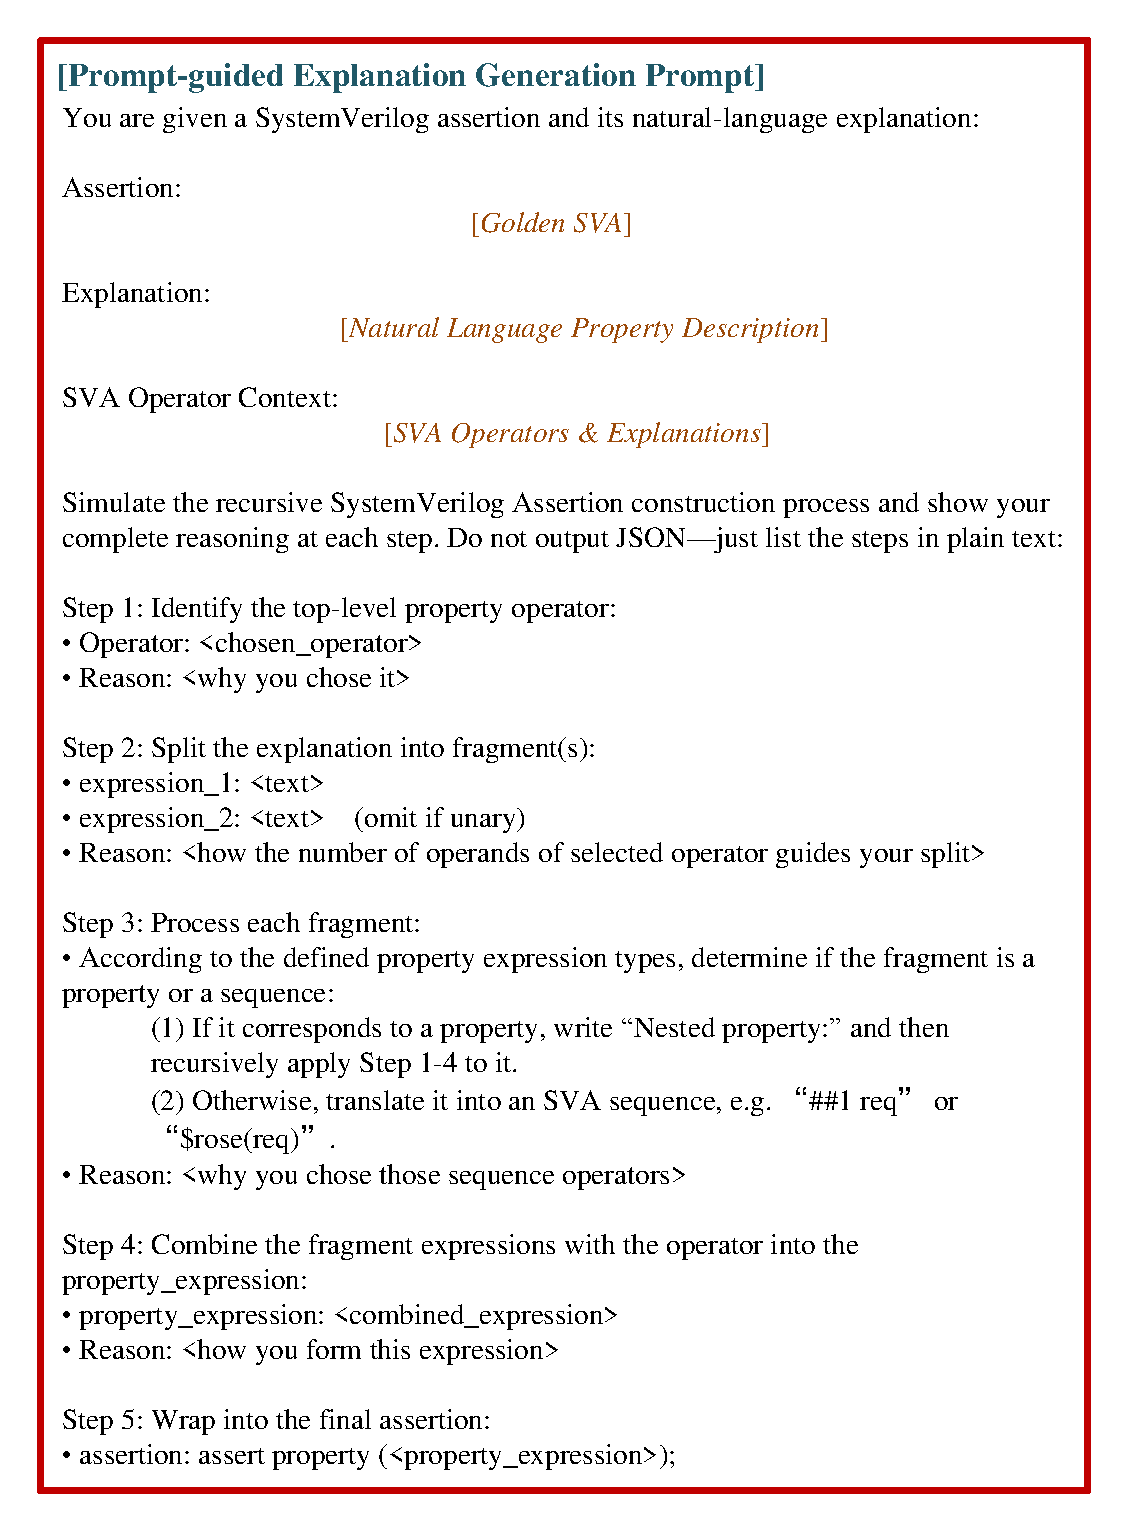
\includegraphics[width=0.6\linewidth]{Figs/Prompt-guided-Explanation-Generation.pdf}
    \caption{Prompt for generating the prompt-guided explanation.}
    \label{fig:prompt-guided-explanation-generation}
\end{figure}

\subsection{Example Prompt-guided Explanation}
\label{subsec:example-prompt-guided-explanation}
Golden SVA:
\begin{verbatim}
    @(posedge pclk) refSig |-> $stable(StableSig)
\end{verbatim}
Natural language explanation:

A property expression that for every rising edge of the clock at which a given reference signal \texttt{refSig} is true, the stable‐value check on another signal \texttt{StableSig} succeeds in that same cycle.
\\
\\
The corresponding prompt-guided explanation is shown in Fig.~\ref{fig:example-prompt-guided-explanation}, which is generated by OpenAI o4-mini.
\begin{figure}
    \centering
    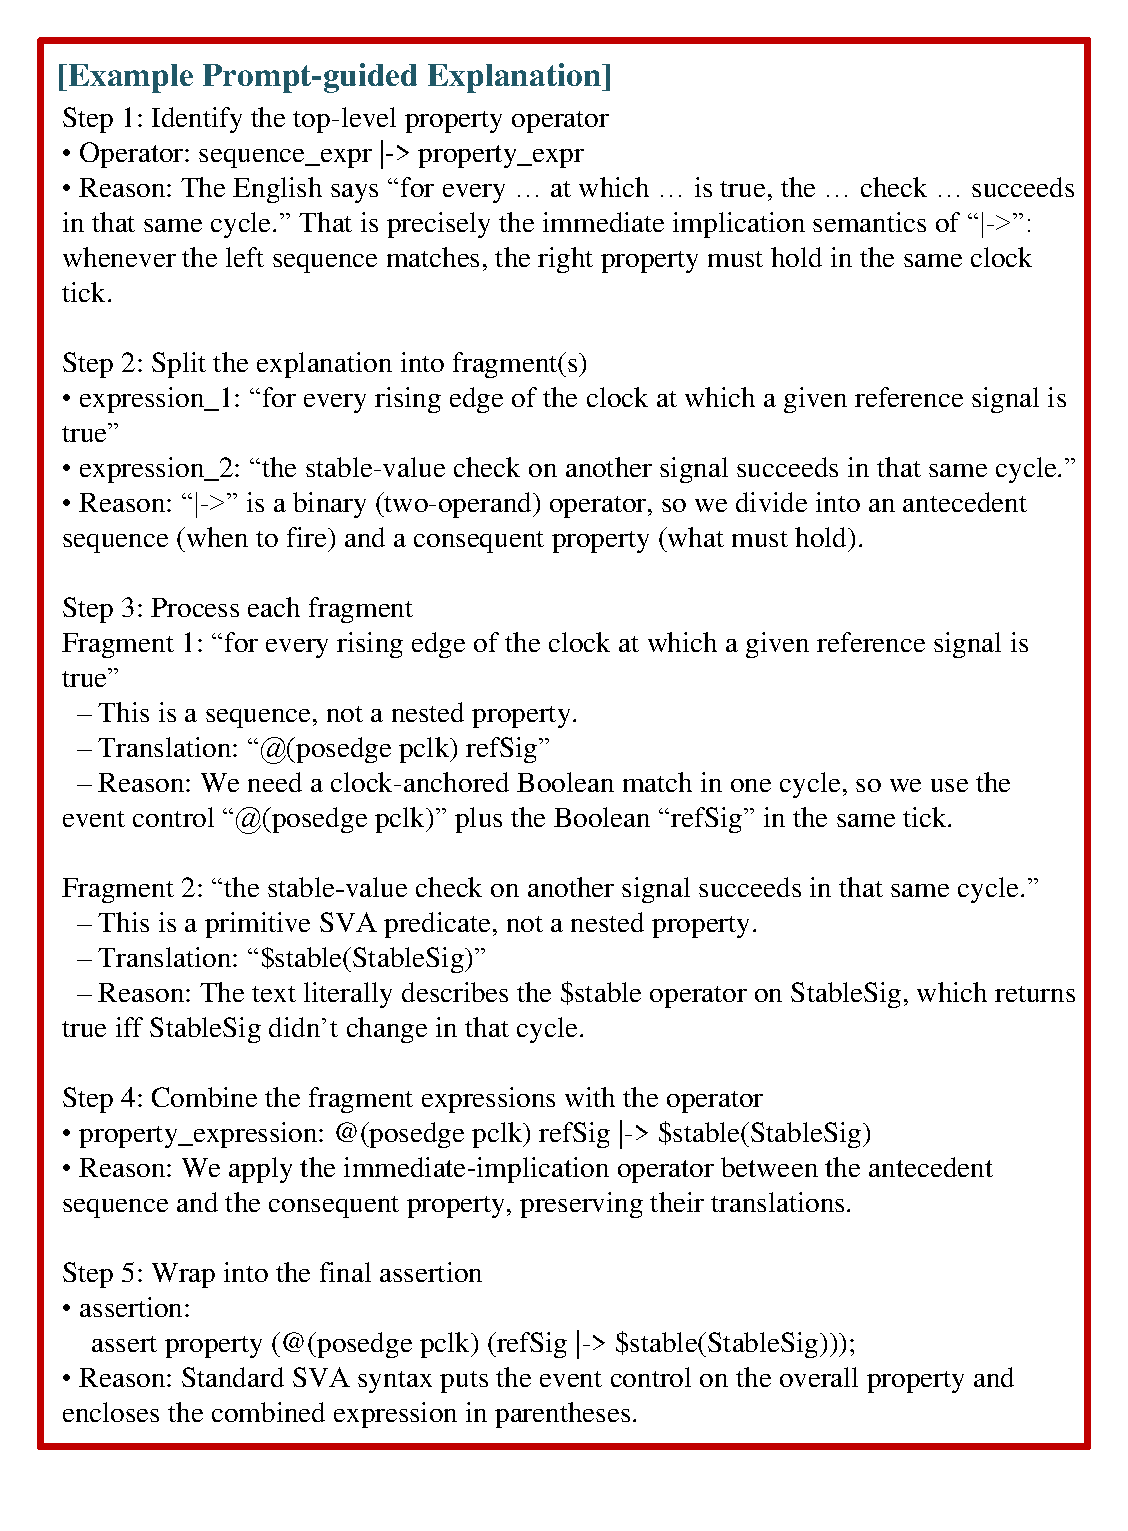
\includegraphics[width=0.6\linewidth]{Figs/Example-Prompt-Guided-Explanation.pdf}
    \caption{An example prompt-guided explanation.}
    \label{fig:example-prompt-guided-explanation}
\end{figure}








\end{document}
